\chapter{Aror}
\label{sec:Aror}

The world of Everblack is situated on a small planet that is called Aror. Aror
rotates around a binary star system we call Carinae. Both suns can be seen on
the sky, with one being slightly smaller than the other.

The planet also has two moons, one of which is named Lilest and the other
Storst, in honour of the two magi that first identified most of the celestial
bodies in our solar sytem. They have many different names in different
cultures and languages, but the names Lilest and Storst are always understood
to refer to the two moons in the night sky.

Aror takes roughly twenty-four (24) hours to rotate around its own axis, while
Lilest goes around the planet in thirty-two (32) days, the bigger moon Storst
takes forty-eight (48) days to make one trip around Aror. Aror itself takes
385 days to travel around the binary star constellation.

Aror is not alone in the system. It is in fact the third planet from the
suns. The first, we call Forun, and is a molten rock of magma, insane
temperatures and poisonous gases. Parin is seated between Forun and Aror, and
can be seen with the naked eye on a clear night sky as a blue shimmering
light. Then follow Ivir and Novar which are believed to be huge planets made
of various gases. Far beyond the reaches of Novar is Piad a smaller, rocky
planet on the edge of our binary star system.

% Geography of Aror
\section{Geography of Aror}
\label{sec:Geography}

The land of Aror encompasses eight great continents, of which all but one are
inhabited by sentient races. The planet has two polar ice caps, as well as lush
rainforests around the equator. Both the northern and southern hemispheres
experience moderate to cold climate depending on the latitude. Latitude 0 runs
through what has been determined to be central island in the middle of the
archipelago known as the \nameref{sec:Silver Isles}.

\subsection{Arania}
\label{sec:Arania}

To the west of Karnak, and in the south western corner of Aror lies the
continent of \emph{Arania}. It is considered the birth place of the ancestors
of all sentient humanoid races, such as the elves, halflings, dwarves and
humans. The continent is a huge and vast steppe, dotted with the occasional
mountain ranges, deserts and fertile oasis. Arania is home to many native and
nomadic tribes, wild animals such as elephants, lions as well as three of the
largest and oldest city kingdoms: \nameref{sec:Fes al-Bashir} to the north
east, and \nameref{sec:Esmayar} and \nameref{sec:El-Fayam}.

In the centre of the continent lies a vast sand desert called the
\nameref{sec:Suam Desert}, which is home to many nomadic tribes of humanoids,
gnolls, hobgoblins, naga, and medusa. South of the desert lies a huge lake,
which feeds many steppes, oasis and other fertile regions surrounding it.

\subsection{Draigynus}
\label{sec:Draigynus}

\emph{Draigynus} is an elongated continent that encircles Farlar to the south
in a half-moon shape. It is close to the southern pale, and thus features a
temperate continental climate to the north, and a subarctic climate to the
south. Very few humanoid races live there, however a small colony of
\hyperref[sec:Dragons]{dragons} has made this continent their home. It is
mostly inhabited by a few sturdy tribes of \hyperref[sec:Snow Elves]{snow
  elves}, and various subarctic beast races.

\subsection{Eilean Mor}
\label{sec:Eilean Mor}

Far to the west, and north of \emph{Arania} lies the continent of \emph{Eilean
  Mor}. It is split in half by a large mountain range called the
\nameref{sec:Great Divide} that runs from all the from the north east down to
the south west. South of the Great Divide lies a vast boreal forest called the
\nameref{sec:Dirgewood}. The continent features subarctic climate in the
north, and temperate climate in the middle, and warmer climate in the
south. Home to many sentient humanoid races, but most predominantly elves,
humans, halflings, and dwarves, it houses four large city kingdoms:
\nameref{sec:Norbury} off the coast in the far north, \nameref{sec:Hraglund}
to the east, \nameref{sec:Helmarnock} to the south east, and
\nameref{sec:Tredegar} to the south west. Eilean Mor is the first continent
that was settled by the humanoid races after the great ice age, and often
referred to as the \emph{old world}.

\subsubsection{Eafiadir}
\label{sec:Eafiadir}

North of Eilean Mor lies a massive dormant volcano called \emph{Eafiadir}. It
is the source of many rivers, and is surrounded by many poisonous sulphur pits
and lakes. Although the area around the volcano is more sparsely populated
there are many smaller baronies and kingdoms on the shores of the north and
north west of the mountain.

\subsection{Farlar}
\label{sec:Farlar}

South of Goltir lies the smaller continent of \emph{Farlar}. Known for its
diverse biome and hilly country side in the north, and cold tundra in the
south. It is now home to mostly \hyperref[sec:Giants]{giants}, giant races
such as ogres and trolls, and also \hyperref[sec:Diarim]{diarim}. The north is
covered with thick and lush forests, which are watered by several large
streams and lakes. These lakes and streams are fed by the fresh rainfall that
falls against the mountain range called \emph{Lias'wa}. The mountain range
splits the continent in half, and allows for a colder climate in the southern
part of the continent. Among all the continents Farlar is by far the smallest,
and once housed the sprawling city kingdom of \emph{Nen-Hilith} before the
giants forcefully took the land as their own.

\subsection{Goltir}
\label{sec:Goltir}

The largest and westernmost continent of Aror, named \emph{Goltir} stretches
from the northern polar ice caps beyond the equator. It is separated in two
large landmasses by a mountain range called \emph{Torainn}. Although the
entire continent is called Goltir, it is often divided into north and south
Goltir, split east to west by the Torainn mountain range.

North Goltir is the home of the city kingdoms of \nameref{sec:Forsby},
\nameref{sec:Kesmar} and \nameref{sec:Stenheim}. North Goltir also known as
the ``land of lakes'' as its entire central landmass is dotted with millions
of smaller lakes, rivers and springs. The central area between Kesmar and
Forsby is called the \emph{Toralian} highlands, and is ruled by various smaller
baronies, earldoms and individual tribes.

A mountain range called the \emph{Alparan} mountains stretches from the centre
to north east, reaching into the polar ice cap of the northern pale. In the
west, the continent stretches out a land tongue towards the Silver Isles,
which was responsible for allowing the early humanoids to spread to the
archipelago. To the south the continent features a vast sand desert, called
the \emph{Walusian Desert} that reaches the foot of the mountain chain
\emph{Torainn}.

North Goltir is home to many sentient humanoid as well as beast races. Humans,
halflings, elves and dwarves live in small baronies in the moderate climate of
the central regions. They share their land with tribes of orcs, bugbears,
hobgoblin, goblins, ogres, trolls, and gnolls who prefer the desert region of
the south.

\subsubsection{Cnámh Mountains}
\label{sec:Cnamh Mountains}

The Cnámh mountain range resides on the eastern shores of North Goltir. They
run from the central regions of the Torlian highlands all the way east towards
the great sea. The mountain range is famous for housing the
\hyperref[sec:Kesmar]{Blackhammer Clan} the biggest and oldest dwarven clan on
all of Aror. South of the mountain range, along a river fed by the mountains,
lies the city of \nameref{sec:Kesmar}.

\subsubsection{South Goltir}
\label{sec:South Goltir}

South of the mountain range of \emph{Torainn} lies the continent \emph{South
  Goltir}. From the mountain range southward it is mostly steppe and grassland
but turns into a thick rainforest around the equator. The most prominent
feature is the almost 9000 metre high \emph{Goban} mountain that peeks forth
from the impenetrable rainforest. The mountain is also the source of the
\emph{Al'ahri} river that runs all the way south through the rainforest, the
southern desert into the sea. The desert and jungle are mostly inhabited by
native and nomadic tribes of elves, monstrous races, as well as certain beast
races such as harpies and gorgons. Gnolls and nomadic humanoid tribes roam the
desert, while the far south hosts the city kingdom of \emph{Avenfjord}.

\subsubsection{Goban}
\label{sec:Goban}

Goban is a large mountain peak that towers above a smaller mountain range in
the centre of southern Goltir. With a size of roughly 9000 metres, it is the
largest mountain on all of Aror. It is the origin of many rivers that worm
their way through southern Goltir, making the land surrounding the mountain
fertile and humid.

Just north of the mountain, and south of Torainn, is also a vast grassland and
jungle called \emph{Goban Jungle}. It is fuelled by the many rivers and their
side arms that spring forth from both the Torainn and Goban mountain range.
The jungle is home to many exotic animals, various tribes of both humanoid and
monstrous races, as well as many elusive and exotic beast races.

South of the mountain is a vast sand desert, called the \emph{Goban desert}.
It features a few fertile oasis and grass lands, but is mostly an inhospitable
sea of sand and heat. Many nomadic humanoid tribes (especially halflings), as
well as many nomadic monstrous tribes (such as gnolls, hobgoblins and ogres)
call this desert their home.

\subsection{Iâfandir}
\label{sec:Iafandir}

Far to the north west lies the continent of \emph{Iâfandir}. It is often
called the \emph{savage lands}, because of its harsh subarctic climate, cold
winters, and the many beasts and beast races that call it home. Most of the
civilisations and tribes there live on the shores along the southern bank, as
the land becomes a frozen tundra further north. It is home of many
\hyperref[sec:Snow Elves]{snow elves} and the \nameref{sec:Tynrikke}, as well as
various monstrous races such as ogres, trolls and hobgoblins, it became
synonymous with a cold climate, harsh conditions and a primal, more savage way
of living.

Although only populated by smaller tribes, villages and perhaps the occasional
snow elven or hobgoblin city, the continent was the birth place of the youngest
city kingdom on Aror: \nameref{sec:Morkan}.

\subsection{Karnak}
\label{sec:Karnak}

West of the land of the dragons is the massive continent of \emph{Karnak}.The
continent itself features a massive lake in its centre, called \emph{Mu'ut}.
The lake is encased in huge mountain ranges, and mostly inaccessible by
land. The lake itself is considered holy to many of the native tribes of the
continent, and is also the home of an ancient evil god called
\nameref{sec:Xir}.

The northern, eastern and western parts of the continent are covered in a vast
and untouched rain forest called \nameref{sec:Yuacata}. The continent is
mostly inhabited by a vast amount of small tribes of wood elves, beast races
such as gorgons, harpies and many different and often dangerous animals such
as apes, primates, tigers and jaguars.

It has a vast chain of large islands off the northern coast, which are mostly
covered in rain forests, called the \emph{Kanaria Archipelago}. It houses many
native tribes but is also home to many smaller outposts of various trading
guilds, mining corporations, slavers and pirates, that exploit the archipelago
for its resources.

\subsection{Silver Isles}

In the centre of the vast sea that separates all the continent, stretching in
from the land tongue of \emph{North Goltir}, lies the archipelago called the
\nameref{sec:Silver Isles}. A huge network of thousands of smaller islands and
inlets, which are mostly covered with rain forests and jungles. It is the
native home of many beasts, native tribes as well as newly settled villages
and expeditions that seek to find what the islands are named after: mineral
riches.


% General explanation on time keeping on Aror
\section{Time Keeping}

A year on \emph{Aror} takes roughly 385 days. Years are prefixed with an
\emph{Aeon}, which are only changed in case of a world-shattering event
or shift, or in case the year numbers become unwieldy. As of the last
edit of this book, the current Aeon prefix is \emph{MI} which stands for
the Aeon of Midaris. In official records you will also find prefixes for
which calendar is used. For example \emph{S/20/05 MI:2002} denotes the
twentieth day of the fifth month in the year 2002 in the Aeon of
Midaris, as described by the \emph{Storst} calendar.

The last \emph{aeon} is now called ``gamla tiden'' (or the ``old age'' in old
teranim), and it began almost three and half thousand years ago (3411 to be
precise). Its prefix is \emph{GT}.

\subsection{Old Calendar}
\label{sec:Old Calendar}

If you use the orbit of the bigger moon \emph{Lilest} to create a
calendar, you get twelve (12) months, with thirty-two (32) days
each. A month is then often broken down to four (4) weeks with eight
(8) days each. Although the \emph{Lilest} based calendar was used
preliminary in the norther hemisphere, it has fallen out of favour and
has been replaced with the \emph{Storst} calendar by MI:1000. Many
cultures still use the old calendar, but most cultures of relevance
have made the switch to the new calendar.

\subsection{New Calendar}
\label{sec:New Calendar}

A calendar utilising the rotation of the moon \emph{Storst} is favoured
in the southern hemisphere. Since most arcane and scientific studies are
done in the southern hemisphere, it has been the de facto calendar of all
of Aror since a few decades.

It separates the year into eight (8) months, with forty-eight (48) days
each, which is then again subdivided into four months with twelve (12)
days each.


% And history, full with timeline
\section{History of the World}
\label{sec:History}

\subsection{Early History}

Roughly sixty thousand years ago an ice age covered most of the world
of \emph{Aror} in vast sheets of ice and snow. Continents that were separated
by sea, where now suddenly accessible through thick sheets of ice. This
allowed the \textbf{four core humanoid races}, the
\hyperref[sec:Humans]{humans}, \hyperref[sec:Elves]{elves},
\hyperref[sec:Dwarves]{dwarves} and \hyperref[sec:Halflings]{halflings}
to migrate away from \nameref{sec:Arania} and settle the entire known
world. Although the humanoid races were successful in adapting to the new
lands and challenges, they had to face fierce opposition.

\subsection{Aeon of Strife}
\label{sec:Aeon of Strife}

When the humanoid races arrived in the other continents around a thousands of
years before the aeon of \emph{GT}, they found that they were already
inhabited by sentient races. \textbf{Monstrous races} such as ogres,
minotaurs, orcs, trolls, hobgoblins, gnolls, bugbears already called these
continents their home, alongside non-sentient monstrous species such as
hydras, manticores and wyverns. Through ancient stories of the dwarves, early
writings, ancient stone tablets, tales from the \hyperref[sec:Dragons]{dragons},
and even cave paintings, it was revealed that the humanoid ancestors were in a
constant state of conflict with these monstrous races. Wars, skirmishes, and
often the destruction of entire early villages and even cities was a common
occurrence in early history. This early time of constant fighting, turmoil and
wars against the sentient beast races is now referred to as the \emph{aeon of
  strife}.

The aeon saw the birth of many new races, such as
\hyperref[sec:Vampires]{vampires}, \hyperref[sec:Fey]{fey} and
\hyperref[sec:Lycanthropes]{lycanthropes}. It also saw a vast destruction of
nature, as both sides of the war cut down forests, dried swamps, and forever
corrupted landscapes and areas with dark and foul magic. The aeon of strife
lasted well into the aeon of \emph{GT}.

Even though the aeon of strife is now hundreds of years in the past, it is
still vividly remembered in both humanoid and monstrous cultures through
stories, song, and tradition.

\subsection{Schism}
\label{sec:Schism}

The ultimately successful survival strategy to deal with such a hostility
during the strife ingrained itself as the cultural core of the humanoid
races. The dwarves went underground and organised themselves in strict
hierarchical clans and cities, that allowed them to optimise their economies to
the harsh realities and lack of resources of the depths. Some humans and elves
followed the dwarves underground but ultimately failed to replicate the
dwarven's success. With a few notable exceptions such as \nameref{sec:Stenheim}.
Although the \nameref{sec:Deepkin}, the underground dwelling cousins of the
humans, built large civilisations underground they were ultimately defeated by
the sentient races of the depths and driven to the surface. The dark elves
instead relied on small clans, families and by being constantly on the move to
ensure the survival of their species.

Meanwhile on the surface elves and halflings sought to settle as far away from
the monstrous races as possible, leading them to the continent of \emph{South
Goltir} and \emph{Farlar}. Other elves settled in the frozen north and south,
becoming known as the \nameref{sec:Snow Elves}. Humans on the other hand used
their ingenuity and skill to build great civilisations and cities that could
potentially withstand the skirmishes and sieges of the sentient monstrous
races. Through many iterations over the course of thousands of years, which
resulted in countless destroyed and ransacked cities and fallen civilisations,
humans have now achieved the unthinkable: dethrone the monstrous races as the
predominant species across all of Aror.

\subsection{Exodus from the Depths}
\label{sec:Exodus from the Depths}

Now many elves and halflings have joined the human effort of building large
centres of civilisation, enriching the predominantly human city kingdoms that
dot the world of \emph{Aror}. Their struggle against the sentient monstrous
races is far from over, especially in the central regions of the continents,
or from the still predominantly monstrous continent of \emph{Iâfandir}. The
majority of dwarves have remained underground, continuing their strict ways of
life as it has served them for aeons. A success that was not shared by the
dark elves and deepkin, who have mostly abandoned the deep and returned to the
surface.

\subsection{First City Kingdoms}

The tide of the aeon long war against the monstrous humanoids turned in favour
for the humanoid races when the first large city kingdoms were founded. These
huge and vast cities provided defence, security and above else a place where
society, culture, and means of production could grow and flourish. The first
city kingdom to be founded was \nameref{sec:Fes al-Bashir}, and its success
in the battles during the aeon of strife, was soon copied across the world.
The early years of what is now the the aeon of \emph{GT}, saw the formation
of many powerful nations, such as \nameref{sec:Hraglund}, \nameref{sec:Esmayar}
and \nameref{sec:Helmarnock}, which helped cement the humanoid victory and
conquest with brick and stone.


% Special note on slavery
\section{Slavery}
\label{sec:Slavery}

Slavery is a sad reality among many city kingdoms, nations, baronies and
tribes of Aror. Many nations and kingdoms allow their citizens to own
sentient monstrous races, or even other humanoids. Slaves often do
hard and menial labour, or even more dangerous tasks such as fighting
as front line troops, work in extreme conditions, or mine the poisonous
\hyperref[sec:Everblack]{everblack}.

To many of these city kingdoms slavery is an integral part to the economy,
and the economic pressure to keep maintaining such an inhumane system
is relatively high. For example \nameref{sec:El-Fayam} would not be able
to flourish, without the slaves toiling away beneath the city to mine
the dangerously toxic everblack.

In most of these systems the slave is nothing more than property. A slave
can be sold, purchased, stolen and property damage is to be paid should
someone hurt the slave of another. The detailed laws may vary based on
the specific kingdom and nation, but often recognise the right of citizens
of another nations to their slaves.

Almost all slaves are registered similar to citizens and there are often
official organisations involved in trading, capturing, and tracking down
slaves that have fled. One such organisation is the \nameref{sec:Hunters
  Guild} of \nameref{sec:Norbury}, or the \nameref{sec:Velvet Hand} of
\nameref{sec:Fes al-Bashir}. These organisations often hire slave hunters,
slavers, task masters and other personnel required to maintain the slave
system within a city. They also offer administrative services, such as looking
up slave registrations, transfers of ownerships and often operate slave
markets and auctions where new slaves are sold.

All slaves are marked as such but the methods vary greatly. Some slaves
are just branded as slaves, often behind the ear or at the back of neck.
Other kingdoms use more sophisticated measures, such as the
\nameref{sec:Slave Band} or \nameref{sec:Slave Mark}. These magical
chains are then often keyed to one or more \nameref{sec:Master Ring} which
are worn by the owners of the slave.

\subsection{Indentured Servitude}
\label{sec:Indentured Servitude}

The system of indentured servitude is practised in many city states, even
those that ban slavery. It is a punishment often placed upon criminals found
guilty of property crimes such as property damage, theft or defaulting on
debts. The criminal is convicted, and then forced to work off his damage in
service to the person or institution to whom the damage was done. These
punishments are often limited in time, but may result in actual prison
sentences if the convict attempts to flee from his duties.

\subsection{Regulated Slavery}
\label{sec:Regulated Slavery}

It also varies greatly between the nations and city kingdoms how slavery is
encoded by law. Most city kingdoms do have laws regarding the treatment of
slaves, such as requiring them to be fed and clothed, or inflicting punishment
to owners should they wilfully neglect or kill their own slaves. Some systems
even encode conditions how children of slaves are to be treated, and whether
they are free or not. And often also encode conditions on how a slave can free
themselves from their bondage. This form of slavery is often called
\emph{regulated slavery}. This system is practised in \nameref{sec:Helmarnock}
and \nameref{sec:Kesmar}.

\subsection{Unregulated Slavery}
\label{sec:Unregulated Slavery}

A rather rare form of slavery is \emph{unregulated slavery}. In this legal
system slaves have no rights whatsoever, and are the complete mercy of their
owner. They are still counted as property within the legal system, and thus
can be sold and bought. But the owner has no obligations towards the slave.
This system is practised in \nameref{sec:Norbury} as well as
\nameref{sec:Morkan}, and by the gnolls of \nameref{sec:Esmayar}.

\subsection{Vonir Accord}
\label{sec:Vonir Accord}

The \emph{Vonir Accord}, named after king Sigmund Vonirson of Norbury, is a
treaty signed by almost all major city kingdoms and most bigger baronies of
the north. In exchange for immunity to enslavement of the signing parties'
citizens, all Norbury slaves found on foreign soil must be returned to
Norbury. Further all signing parties must acknowledge the owner's claim over
his slave and not interfere with his rights to his property. This treaty
also allows members of the \nameref{sec:Hunters Guild} to search for, and
apprehend escaped slaves on the land of signing parties.


% Globalism
\section{A Global World}

The world of \hyperref[sec:Aror]{Aror} has a few major city kingdoms that are
vastly populated centres of society and civilisation. These immense cities are
the major power players in the world, and often have power over the fates of
many million people. Not only in their own realm, but also in the lands,
baronies and smaller kingdoms they project their power onto.

Knowledge about the other city kingdoms is wide spread, and almost all people
have a rough understanding on how big the world is, and what culture lives
where. Although travel is only feasible for the middle and upper classes, word
about foreign lands and the intricate politics of the city kingdoms spreads
easily to every corner of the land.

\subsection{Dragon Teleporter}
\label{sec:Dragon Teleporter}

These large city kingdoms are also connected with each other with large
teleporters, that were originally invented by the dragons to inter connect
places of interest on their continent of \nameref{sec:Draigynus}. A dragon
teleporter has three large pillars, that sharpen to a point at their end. They
are arranged in a circle that arch inward, touching each other at the top, to
form a sort of arch over a small area beneath them. Once activated arcane
energy flows from their stem to the tip, where they form a glowing, floating
ball of energy beneath the arch, that acts as the horizon for the
teleportation magic. Once a living person touches the horizon, they are
instantly transported near one of the pillars of the remote teleporter. A
teleporter that receives a person, can still teleport one other person away at
the same time.

Draconic runes are inscribed into the pillar and help with selecting a target
for the teleportation, and can be used to program new targets into an existing
teleporter. A dragon teleporter requires considerable arcane power to operate,
and can only teleport one person at a time to a another, preprogrammed, dragon
teleporter. It may still receive another visitor at the same time as it sends
another traveller to a distant teleporter.

In \emph{MI:782} one of these dragon teleporters was found in the depths of
the \nameref{sec:Great Divide} by a mining expedition. It was reverse
engineered by arcane scholars and wizards and then installed in all city
kingdoms that could afford to buy and maintain one. Now they are often seated
centrally within the kingdom, and everyone can purchase tickets to be
transported to another city kingdom of their choosing. Prices for tickets
often range from five to twenty \hyperref[sec:Shin]{shins}, depending on the
prices of the city kingdom. For almost all city kingdoms the teleporters are a
net loss commercially, but they are aware that the trade and commerce (and
thus taxes) they help facilitate is invaluable to the economy of the kingdom.

This lead to the large city kingdoms to become more and more interconnected.
It helped spread the clean, high version of \emph{Teranim} to be spoken all
over the world, as a lingua franca was required to facilitate trade and
commerce.

The dragon teleporters were designed to transport living creatures (dragons)
across great distances, and are almost incapable of transporting material
goods. One teleport can transport one person plus their light equipment, or
perhaps ten kilograms of innate material (such as armour, weapons and
clothes) at a time. This design choice was deliberate by the dragons, as they
do not wear or own that much innate objects; and thus have designed their
teleporters to transport themselves safely and efficiently across vast
distances.

Many have feared that the trade by sea or land would become obsolete since
teleporters were introduced. But the dragons did not share their blueprints,
and the knowledge about the dragon teleporters is still actively researched
and reverse engineered to this day. Their design limitation and relatively
high power consumption has made them a bad economical alternative for
transporting goods.

\subsection{Global Trade}
\label{sec:Trade}

All city kingdoms and the majority of baronies mint their own coins, but they
are often only used locally. Although their value is held by precious metals
they contain, they have a strong variance in terms of metal purity, weight and
thus actual value. This made conversion of one local coin or currency to
another difficult. To make global trade and commerce easier, two new
currencies were introduces: the \emph{shin} and the \emph{shard} which are
made out of \hyperref[sec:Everblack]{everblack}.

Many banks offer a service to weigh, assess and convert local coins and
gemstones to shin and shard. And almost all baronies and kingdoms accept shins
and shards as payment method. Large purchases, such as properties or ships, are
mostly done in shards, or perhaps in bars of pure gold. Although crystal
everblack is more easily shattered and destroyed than gold, it is lighter
to carry and it cannot be as easily diluted or forged. Manipulating everblack
takes a highly skilled arcane wielder or scientific scholar, and thus cannot
be forged or manipulated like other ore or metals.

Thus many traders might simply refuse to take foreign coin, or even local
coins, preferring to deal with the more save shins and shards of everblack.
Assessing the purity of large amounts of gold or silver coins can be costly
and time consuming, and thus traders that deal with expensive items might
prefer the safety and convenience of the everblack based currency.

\subsubsection{Shin}
\label{sec:Shin}

Small chips of \hyperref[sec:Everblack]{everblack}, roughly a centimetre in
diameter - also referred to as \emph{shins} - are a common currency accepted
everywhere on the world of Aror. These are often useless for magical
applications due to their small size, but still hold material value. They are
roughly equivalent to one copper coin and are used to make everyday purchases.

\subsubsection{Shard}
\label{sec:Shard}

Bigger sticks of everblack, roughly five centimetres long, one centimetre thick
and perhaps one centimetre wide are called \emph{shards}. They are used in the
global economy of Aror for expensive purchases such as building projects,
property and artefacts. Shards are roughly equivalent to ten coins of gold.


% Maladies
\section{Afflictions}
\label{sec:Afflictions}

Aror is not only home to various dangerous races, but also to various
maladies, sicknesses, and diseases that may be dangerous to you. Should you be
an inter-planar traveller and show any symptoms listed here, you best consult
a priest, cleric or a follower of \nameref{sec:Ishtar}. The authors of this
book are not competent enough to give medical advise.

\subsection{Black Blight}
\label{sec:Black Blight}

The \emph{Black Blight} (black pest, or miner's disease) is a living,
poisonous organism that is capable of infecting any living creature. The
blight exists as a black gooey liquid beneath the surface, and once it has
sensed heat emanating from a living being, it will slowly move towards the
source in an attempt to infect the creature. Its most dangerous when dissolved
in underwater lakes, as only a few drops are sufficient to infect a
human-sized creature, or when stuck to cave ceilings as it can drop itself
down onto unsuspecting cave explorers.

Once a creature has been infected it will show symptoms of the common flu:
head ache, cough, sore limbs, fever and running nose. The blight is thus
often mistaken for the common cold, and not treated any further. At this
stage of the blight, strict bed rest, and a strict medicinal regimen from
a doctor can defeat the blight before it causes any more damage.

However if it remains untreated the blight moves on to stage two within ten
days or a week. Those infected will begin to lose their grasp on memory,
become delusional, experience hallucinations, until ultimately, they become
feral and aggressive within two weeks. Once this stage has been reached the
infected become ``blight bearers'', who can easily transmit the disease to
others with scratches, bites, or exchange of fluids. Blight bearers are
exceedingly dangerous within the confines of cities, as they can easily infect
hundreds of people by contaminating wells with their blood. A blight bearer
can only be stopped by killing them, and burning their bodies to destroy
the disease.

In \emph{MI:1680} a single blight bearer was responsible for the death of
roughly 12 million people in, and surrounding the city of
\nameref{sec:Hraglund}. The initially infected people were masked beneath a
wave of genuine influenza infections, and the rapid spread of the blight
remained largely unnoticed until it was too late. Lessons were learned from
the tragedy, as major centres of civilisation now mandate regular health
checks for miners, adventurers, and other professions of risk at becoming
infected with the blight. Most city kingdoms offer the cure of stage one
blight for free, should it be diagnosed by a doctor, or a priest.

\subsection{Rot}
\label{sec:Rot}

The ``rot'' or ``black rot'' is a disease that most people of Aror get during
their early childhood. Its first stage is harmless, with sore, and flaking
skin around the toes, fingers, and the nose and mouth. If the child is strong
enough the disease will never progress any further, and disappear after one or
two weeks. In such a case the child has been immunised against the black rot
for the rest of its life.

In rare cases however, especially in weak, malnourished children or those that
already suffer another disease at the same time, the disease will advance to
stage two, and begin to fester and spread. The skin of the diseased will begin
to peel, the flesh turns black, and ultimately rot, causing immense pain, and
suffering. The severity of the disease varies greatly. In mild cases only one
hand or foot is affected, while severe cases have it in all or most limbs,
allowing them to live for decades before the disease becomes fatal. Those
unfortunate enough to have the rot fester in the face have only a few years to
life, as nourishing yourself becomes ever more difficult. The last stage of
the black root is ultimately fatal, as over the course of years the disease
will spread from the extremities towards the torso, ultimately infecting major
organs.

A herbal medicine exists for stage one rot, which is readily available in
alchemy stores. But no natural medicine or treatment exists for the second
stage of the disease. Those afflicted with the advanced stage of the black rot
are usually invalid, relying on others to provide for them, as motor functions
are severely limited in the affected limbs.

\begin{35e}{Rot}
  The disease \emph{Rot} has DC12, and causes 1d4 points of \emph{dexterity}
  and \emph{charisma} damage. If untreated the disease will advance to stage
  two within two weeks, causing 1d6 \emph{dexterity} drain, and 1d6
  \emph{charisma} drain.

  Stage one rot can easily be cured by succeeding a \emph{Survival} check DC15
  to find the correct herb, and a \emph{Craft Alchemy} check DC13 to brew a
  tea from it. The herb is readily available in well-sorted alchemy stores.
\end{35e}

\subsection{Troll Blood}
\label{sec:Troll Blood}

The monstrous creatures of the species troll have remarkable self regeneration
powers, that make them dangerous opponents. They achieve this remarkable feat
through their blood, which in itself is one of the most toxic substances on
Aror. Troll blood accelerates natural growth in any animal, plant, creature,
or humanoid in comes in contact with, but the effects are only beneficial to
trolls. Any other organism exposed to troll blood will find the effected area
to start growing wildly, and rapidly often leading to horrible deformations,
cancerous growths, and very often to death.

In the early centuries of the strife it was common to see warriors, hunters,
and soldiers with deformities, cancerous growths, and horribly deformed bodies
due to exposure to troll blood. Troll blood affects any living creature, and
so both monstrous and humanoid clans and tribes tried to either drive trolls
away, or outright kill them in an effort to limit the damage they could do with
their blood. Fire, and acid are effective treatments against the mutations, as
is amputation of the effected areas.

Nowadays (starting with \emph{MI:0}) trolls have become increasingly rare, and
so have deformities or death due to exposure to troll blood. If trolls are
discovered to be living in area, it is highly advised to call upon the aid of
the \nameref{sec:Wayfaerers Guild}.

\begin{35e}{Troll Blood}
  Troll Blood lead to random deformities, cancerous growths and perhaps even
  death if people are exposed to it. Wounding a troll in melee risks exposure,
  and only a reflex save (DC: 5 + damage done) allows one to avoid exposure to
  the trolls blood. Effect of troll blood can be resisted (fortitude save DC:
  10 + $ frac{1}{2} $ HD + \emph{CON} modifier), and the results are random
  but almost never pleasant. Both fire and acid can counter act mutations from
  troll blood, as does amputation of an effected area or limb.
\end{35e}


% City Kingdoms
\section{City Kingdoms}
\label{sec:City Kingdoms}

The world of \emph{Aror} is covered in a few huge and ancient human kingdoms
that exert their influence and power from vast cities. These cities often
house millions of humanoid creatures, and the kingdom's influence and power
extended outward to surrounding areas. Most of these cities are sprawling
metropolises that house an overwhelming amount of humanoids. The populations
listed here include any surrounding area, smaller baronies permanently under
the kingdom's control, and even outlying cities that fall under the
jurisdiction of the kingdom.

The massive populations of some of these city kingdoms can often only be
sustained through slave labour, and by optimising agriculture through arcane
machinery. Many baronies and aristocratic houses are wealthy and owners of
huge patches of land, who make their fortunes by selling their produce and meat
to the city kingdoms. Small, self sustaining farms are rare close to large
city kingdoms, as they have all been bought up by these huge land barons.
\nameref{sec:House Liares} of Helmarnock is a prime example of a wealthy
aristocratic family that gained their wealth solely by providing the city
kingdom with produce, meat and other agricultural products.

All of these city kingdoms are connected together with \hyperref{sec:Dragon
  Teleporter}{dragon teleporters}, which allows travel and trade between the
kingdoms. They are often a beacon of stability and security. Surrounded by
wild nature, unstable baronies, and small and greedy earldoms that vie for
power and wealth.

Many of these city kingdoms have their own unique culture, local language
dialects, their own laws and customs, and often also unique governments. However
most of these kingdoms are ruled by humans, where other races often take a
secondary role as minorities within the general populace. Still the mixture
of races, backgrounds and various cultures often add a unique touch to the
whole.

In many cases the town or city kingdom you came from defines you more than
your race. A \hyperref[sec:Snow Elves]{snow elf} born in
\nameref{sec:Avenfjord} will have grown up with that cities culture, most
likely favouring the arts over the hunting bow. Much like a halfling of
\nameref{sec:Norbury} will be a staunch believer of the meritocratic culture
prevalent in the warrior kingdom.

All of these city kingdoms, as well as many bigger baronies, have a system
where they register citizens and also issue official documents to their
citizens. These are often copper rings for common citizens, or even official
documents of identification in case of officials or noble houses. Being a
citizen of one city kingdom not only grants considerable benefits in your
home, but often also grants you special status or privileges in allied city
kingdoms.

The large and vast city kingdoms of the humanoid races take great emphasis
on written documents and record keeping. They also keep a citizen register
within which it all official residents and citizens of the city kingdom are
registered by name, gender, race and age.

Citizens of city kingdoms enjoy additional freedoms within their home nation,
such as the ability to purchase property, found businesses, or own and sell
slaves. Being a citizen of a city nation also offers protection when visiting
other large nations, as many of these cities have mutual protection and
recognition agreements amongst each other that guarantee special wards, such
as protection from enslavement or right to counsel and representation from your
own nation should they be accused of committing crimes.

City nations and kingdoms often issue three types of official identification
papers: \emph{citizen papers}, \hyperref[sec:Citizen Mark]{citizen marks} and
\hyperref[sec:Nobility Mark]{marks of nobility}.

In between most of these city kingdoms stretches out a vast network of smaller
baronies and earldoms. Most of these are too insignificant to mention, and the
unstable nature of small rulings makes tracking them through time a far too
tedious task to be worthwhile for a book of this scope.

\aren{We can perhaps list them all in a separate book. With three thousand
  pages...}

\begin{note}
  The region between city kingdoms is left blank intentionally so that dungeon
  masters and players have leeway to design their own baronies and villages.
\end{note}

%% City Kingdom of Avenfjord
\subsection{Avenfjord}
\label{sec:Avenfjord}

The rebuilt kingdom of the high elves and halflings sits on the southern shore
of the continent of \nameref{sec:Goltir}. It settled in the vast and fertile
river delta of the \emph{Al'ahri} river. Avenfjord is one of the youngest of
all the city kingdoms, and also the smallest.

\subsubsection{Banner}

The banner of Avenfjord depicts two large crowned towers built together by
a bridge, with a backdrop of blue (for the sea) and green (for the fertile
farm land).

\subsubsection{History}
\label{sec:Nen-Hilith}

It was founded in MI:1920 when the giants, an extra planar race of towering
humanoids, destroyed the previous city of the halflings and elves called
\emph{Nen-Hilith}. They had invaded the continent of \emph{Farlar} thirty
years prior, to wage war against the dragons who also call that continent
their home. \emph{Nen-Hilith} was situated on the northern shores of
\emph{Farlar} (just across the sea from where Avenfjord stands now).

For many years the elves and halflings were untouched and neutral in the
war between the dragons and the giants. But as the giants had seized most of
the rivers and lakes south of \emph{Nen-Hilith} and the fighting had crept
north towards the outlying villages and towns the elves and halflings joined
the war on the side of the dragons in MI:1912. After several failed campaigns
to regain control over the city's water supply, the giants began a devastating
siege against the city in MI:1918. After enduring the siege for more than two
years, with the military aid of various allies, the starved and weakened elves
and halflings were forced to abandon \emph{Nen-Hilith} and flee across the sea
to the north. The giants then razed the city to the ground.

\subsubsection{Formian War}
\label{sec:Formian War}

In MI:1926 a war broke out between a hive of formians who objected to the
elves settling in their lands. The kingdom was still in the early stages of
rebuilding, and the new war threatened the very existence of the nation. The
then ruler of Avenfjord, King Ishmael the II., allowed a travelling wizard
named \emph{Taras} to combat the formians by adapting the \emph{black blight}
to infect and weaken them. Going far beyond anyone's expectation, the modified
plague infected and killed the vast majority of formians living in the Goban
desert north of \emph{Avenfjord}. After realising that he had ordered genocide
upon an entire sentient species \emph{King Ishmael II} exiled \emph{Taras}, who
claimed that he did not know the blight would kill the formians. Later in the
same year King Ishmael II committed suicide. His son \emph{King Ishmael III}
took the throne soon after.

\aren{If he just had enough resolve left to take Taras with him...}

\subsubsection{Culture}

Although one might suspect that the near destruction would shake the culture
of the elves and halflings to the core, you might be wrong. Instead the
formian war, and the destruction of their previous city hardened the nation's
stance of non-interference. The people of Avenfjord prefer not to meddle in
other people's issues and troubles, and prefer diplomatic solutions over
conflict.

Avenfjord are known for their generous patronage for the arts and sciences and
house many theatres, libraries, galleries and workshops. They fund one of the
largest arcane academies on \emph{Aror} and generally hold good relations with
most other city kingdoms. The elves and halflings of Avenfjord are often
described as jovial, carefree but creative and expert diplomats. They are an
open society, and especially welcome other artists and craftsmen into their
cities.

\subsubsection{Population}

The city of Avenfjord is now home to roughly two million people, yet the city
of \emph{Nen-Hilith} was home to almost twenty million at its peak. Most of
the citizens are elves (48\%) and halflings (39\%), with dwarves following
third (8\%) and all other races making up the remaining 5\%.

Common male names are: Aelius, Caius, Felix, Florian, Horatio, Julius, Marcus,
Marius, Otho, Ovid, Senec, Tacitus, Varo, Vitus.

Common female names are: Aelia, Aemilia, Aurelia, Caelia, Cassia, Claudia,
Flavia, Flora, Hadriana, Julia, Lucia, Marina, Paula, Sabina, Titiana,
Valentina, Vita.

\subsubsection{Rule}

Avenfjord is a dual monarchy, where both the reigning king or queen of the
elves, and the reigning monarch of the halflings rule together. Neither of
the monarchs has absolute reign alone. Although Avenfjord holds houses of
nobility, their power and influence is minimal compared to the houses of
other city kingdoms. Slavery and serfdom is outlawed, and all citizens of
Avenfjord are free people. The city also has an independent court and police,
that enact the laws the monarch sign into law fairly.

\subsubsection{Relations}

Avenfjord has not signed the \emph{Vonir Accord} with Norbury. Although this
puts citizens of Avenfjord at risk of enslavement should they travel to
Norbury, such cases are extremely rare. Neither Norbury nor Avenfjord wish
to raise diplomatic issues between the two city kingdoms.

Though traditionally heavily aligned with the city kingdom of Forsby, the
failure to send military aid that was promised during that cities siege
soured relations with most city kingdoms, but with Forsby specifically.

%% City Kingdom of El-Fayam
\cleardoubleevenemptypage

\ifimages
\begin{figure*}[ht!]
  \centering
  \vspace{-5.2cm}
  \centerline{
    \includegraphics[width=\paperwidth,keepaspectratio]{%
      media/elfayam.\imagesuffix
    }
  }
\end{figure*}
\fi

\begin{infobox}{City Kingdom of El-Fayam}
  \ifimages
  \begin{subfigure}[t]{\textwidth}
    \centering
    \includegraphics[width=0.22\linewidth]{%
      media/elfayam-bannersm.\imagesuffix
    }
  \end{subfigure}%
  \fi%
  \begin{multicols}{2}
    \begin{itemize}[label={},noitemsep,leftmargin=0.0cm,topsep=0pt]
      \infoboxitem{Location}{South western shores of \nameref{sec:Arania}
      }
      \infoboxitem{Languages}{Kalest, Teranim, Latas (regional dialect)}
      \infoboxitem{Government}{Absolute Monarchy}
      \infoboxitem{Major Religions}{\nameref{sec:Nyddwr}, \nameref{sec:Forun},
        \nameref{sec:Order}, \nameref{sec:Marwaid}
      }
      \infoboxitem{Area}{est. 50,000 $km^2$}
      \infoboxitem{Population}{est. 900 thousand in total}
      \infoboxitem{Non Grata}{monstrous races (except slaves), devils, druids,
        Gorgons
      }
      \infoboxitem{Magic}{all magic allowed, almost impossible to channel
        magical energy within the city
      }
      \infoboxitem{Slavery}{yes, all forms, overseen by the
        \nameref{sec:Velvet Hand}, used as punishment for criminals, signer
        for the \nameref{sec:Vonir Accord}
      }
      \infoboxitem{Special Laws}{-}
      \infoboxitem{Notable Organisations}{\nameref{sec:House Ranian},
        large auction house of the \nameref{sec:Velvet Hand},
        \nameref{sec:Ror-Aram Trading Corporation}
      }
      \infoboxitem{POI}{Church of \nameref{sec:Lor}, cathedral of the
        \nameref{sec:Order}, large recreational sand beach within the
        city walls, central promenade with many restaurants and shops
      }
    \end{itemize}
  \end{multicols}
\end{infobox}

\clearpage

\subsection{El-Fayam}
\label{sec:El-Fayam}

The city kingdom of \emph{El-Fayam} (``young flower'' in Kalest, also known
as ``Nirum'' in local dialect) lies on the south western shores of
\nameref{sec:Arania}. It was founded in \emph{MI:1260} from the refugees that
had to flee the sacking of \nameref{sec:Esmayar}.

The city's banner features a yellow double headed eagle, upon a light red
background, embedded in a shield upon which rests a crown. The banner was
taken from the old banner of Esmayar. Yellow and red are the city nation's
primary colours.

\subsubsection{History}

The city is one of the youngest on Aror, and was officially recognised as a
city kingdom in MI:1310. It existed as a small fishing village in the oasis of
Nakhmet, but exploded in size after the sacking of Esmayar by the gnolls. Many
of refugees from Esmayar fled to the village and settled there. Soon the small
fishing village became a small town, and ultimately a small kingdom. In
MI:1310 the small kingdom was officially recognised as a city kingdom and
successor in spirit to Esmayar. An act that enraged the gnolls of the northern
neighbours. In MI:1630 the gnolls of Esmayar attempted to besiege and conquer
the city but where ultimately repelled by an alliance of humanoid city
kingdoms.

Many of the new arrivals and refugees were highly skilled labourers and city
builders that helped raise the small village to the status of a prosperous
city and kingdom within a few generations. Over the course of many years the
city expanded into the outlying lands, and thus now owns the vast majority of
the Nakhmet oasis.

\subsubsection{Culture}

The average citizen of El-Fayam enjoys a secure, wealthy live, with many of
the jobs available in the city paying enough to afford a decent living. The
city itself is known for offering many opportunities, both of gifted and skilled
craftsmen, as well as for adventurers. The justice system of the city is fair,
and the guards men pride themselves from keeping order both inside, and outside
of the city. The politicians have learned from the tragedy of Esmayar, and did
not expand the city's sphere of influence beyond what they were able to control,
and secure. Crime in the city is low, although the harbour districts is a hotbed
for smuggling.

The citizens of El-Fayam pray to a wide variety of gods, including
\nameref{sec:Nyddwr}, \nameref{sec:Forun}, \nameref{sec:Marwaid} and the
\nameref{sec:Order}. Although the cultural influence from \nameref{sec:Fes
  al-Bashir} is ever present, the people of El-Fayam are deeply
religious. However tensions from the different believes do arise, they are
very rarely violent.

Many craftsmen from Esmayar took their craft with them, and thus the city is a
mixture of both yellow sandstone, and white brick buildings. The city itself
is known for its delicious food, beautiful scenery, and availability for
luxury goods such as tobacco and coffee.

While the city practices, and allows slavery, the amount of slaves within the
city is low. Most slaves are criminals that toll away their sentences within
the Everblack mines. Most servants to the rich and nobility are serfs, and are
thus not considered property.

The citizens speak a wide variety of languages, including Kalest, Teranim,
Latas (their regional dialect), Enro'ad, and even Rutari.

\subsubsection{Population}

The city kingdom is one of the smallest, being home to roughly 900.000
people all in all. The diversity among the humanoid species is high, with
elves leading slightly (30\%), followed by humans (28\%) and dwarves (22\%)
and then halflings (18\%). Half races and various others make up the remaining
2\%.

Common male names are: Abar, Ahmes, Amosis, Cleo, Hori, Iamesu, Menes,
Merenor, Nedjem, Seneb, Seth, Senec, Takar, Turo, Varo, Yna, Zamon

Common female names are: Aelia, Ahmose, Aurelia, Cleo, Dia, Flora, Herneith,
Kasha, Lysandra, Maia (or Maya), Merita, Nebet, Neth, Pevena, Satiah, Sema,
Tabia

\subsubsection{Imperialism}

After the fall of Esmayar the city was flooded with refugees seeking to build
a new home within the relatively small city's borders. The influx of new
people from the fallen city kingdom catapulted the city from being a minor
player to the most powerful nation in the region. The kingdom not only gained
a highly educated, and skilled workforce, sailors, and ships, but also a
sizeable amount of highly trained, and well equipped veteran warriors from the
siege. It used the warriors to expand its land outwards, seizing most of the
surrounding lands and incorporating it into the newly founded
kingdom. Surrounding monstrous settlements were destroyed, and uncooperative
humanoids were driven from their land. The newly conquered land was then
granted to the refugees for a small administrative fee. After its own
population had been provided with land and opportunities, it began to use its
new army and navy to settle other lands, and islands across Aror. Esmayar now
owns many islands in the \nameref{sec:Kanaria Archipelago}, as well as in the
\nameref{sec:Silver Isles}.

\subsubsection{Luxury}

El-Fayam is the main produces, and exporter of various luxurious goods
including tobacco, chocolate, sugar, coffee, tea, spices
and \nameref{sec:Sarelis}. Combined with its warm climate, friendly and
welcoming people, decadent deserts, readily available slaves as servants, and
beautiful scenery it has gained a reputation as a resort city. The wealthy and
the nobility from all across Aror travel to El-Fayam to indulge, relax, and go
on sabbaticals. The main street, and promenade are filled with coffee shops,
luxury hotels, stores selling luxury items and trinkets, and private houses
that cater to any needs.

\subsubsection{Everblack}

The city kingdom found a large subterranean vein of Everblack in MI:1490
beneath the city while digging and expanding the old village's water drainage
system. An excavation was immediately started, and has now turned into one of
the largest mining operations on Aror. With the new found wealth of selling
the everblack across the world, the city hired skilled labourers, mining
crews, smelters and overseers to continue the massive mining operation.

Although tempted, the city kingdom did not use slave labour to mine beneath
the city, but paid the workers fair wages. But over the course of many
centuries old mining plans were lost, mining shafts collapsed, and the shafts
became home to various subterranean creatures, making the mines beneath the
city's aqueduct a deadly labyrinth. The workers were unwilling to return
there out of fear of being lost or killed. Unable to find any workers willing
to mine the depths beneath the city, the kingdom reinstated slavery in MI:1720
and is now using forced labour to mine the veins in the deep caverns below.

The city kingdom is the main source of everblack on the southern continent,
which made the kingdom unfathomably rich. It has used this wealth to expand
its land, power and influence in the region; as well as continuing to fund
explorations, charting missions and mining operations in the depths beneath
the city in the hopes of finding new veins of Everblack.

Since the city kingdom sits directly on top of so much Everblack, any form
of magic is disrupted within the city. This works both for the city, as
foreign casters cannot do a lot of damage, but also severely restricts any
form of magic research within the city. The city also has a special prison
for magic wielders, that is in high demand around the world.

\begin{note}
  Any form of magic has a 50\% spell failure chance in El-Fayam, and its
  surrounding lands. The spell failure is 75\% within the Everblack mines,
  as trace dust of Everblack absorbs all sorts of magic.
\end{note}

\subsubsection{Culture}

At first the people of El-Fayam were determined to retake their old city as
soon as possible, and thus heavily focused on military and arcane studies in
the early decades of the kingdom's foundation. This view has since shifted after
the discovery of everblack, towards trading, bartering and mining. After
generations having a strong focus on military achievements and pride within
the culture, the values shifted towards wealth and mercantile prowess as well
as arcane study of the black crystal.

Since the ``black gold'' (as it is called in the city) has taken over the main
focus of the kingdom, any measure that aids finding, mining and refining the
black gold has become socially desirable within the city. This culture has
earned the people of El-Fayam a reputation of being ruthless dealers and
businessmen, that would not shy away from introducing slavery to become rich.
The truth however, is that their massive amount of wealth has trickled down
to the people, establishing a large, wealthy and socially stable middle class.

Unlike in other city kingdoms the ruling Malek has very little actual power,
and is seen only as a mere puppet of the mining and trading guilds that
rules the city.

\aren{You will find the people of El-Fayam to be friendly, loving, exceptional
  hosts, always ready and willing to barter with you. Just don't look under
  the metaphorical rug that are their Everblack mines.}

\subsubsection{Relations}

Although still officially an enemy of the new gnoll kingdom of Esmayar, the
kingdom concerns itself little with recapturing its former home. Still it
fights small skirmishes against its northern neighbour, bust mostly to
defend its borders from gnollish incursions.

It holds good relations with Fes al-Bashir, going so far as to invite the Ror
Aram-Trading corporation to help with the selling of the everblack crystals,
as well as inviting the Velvet Hand to oversee slavery within the city. It is
a signer of the \nameref{sec:Vonir Accord} and often trades slaves with both
Fes al-Bashir, Norbury and Helmarnock.

The city kingdom also uses the acquired wealth to simply buy itself into
a good diplomatic standing with anyone that the kingdom deems valuable enough
to have as a friend.

%% City Kingdom of Esmajar
\cleardoubleevenemptypage

%% TODO: Artwork

\begin{infobox}{City Kingdom of El-Fayam}
  %% TODO: Crest
  \begin{multicols}{2}
    \begin{itemize}[label={},noitemsep,leftmargin=0.0cm,topsep=0pt]
      \infoboxitem{Location}{North western shores of \nameref{sec:Arania}
      }
      \infoboxitem{Languages}{Gnoll, Giant}
      \infoboxitem{Government}{Absolute Monarchy}
      \infoboxitem{Major Religions}{\nameref{sec:Three Kings},
        \nameref{sec:Isamir}
      }
      \infoboxitem{Area}{est. 120,000 $km^2$}
      \infoboxitem{Population}{unknown}
      \infoboxitem{Non Grata}{any non-monstrous races without a proper permit
      }
      \infoboxitem{Magic}{all magic banned for non-citizens
      }
      \infoboxitem{Slavery}{yes, all forms}
      \infoboxitem{Special Laws}{unknown}
      \infoboxitem{Notable Organisations}{unknown}
      \infoboxitem{POI}{slave actions, gladiatorial arena, shrine to the
        \nameref{sec:Three Kings}
      }
    \end{itemize}
  \end{multicols}
\end{infobox}

\clearpage

\subsection{Esmayar}
\label{sec:Esmayar}

Esmayar (``white jewel'' in Kalest, also known as ``Arcania'' in local
dialect) was one of the older city kingdoms of Aror, with a rife history but
has since fallen to the gnoll raiders in \emph{MI:1213}. It is located on the
north western shores of \nameref{sec:Arania}.

The city's old humanoid banner featured a yellow double headed eagle, upon a
light red background, embedded in a shield upon which rests a crown. Yellow
and red were the city nation's primary colours.

The new banner shows a dark red head of a gnoll upon white background, beneath
a golden crown. Red, gold and white are the primary colours of the monstrous
kingdom of Esmayar.

\subsubsection{History}

It was founded in \emph{GT:592} in the delta, and along the banks of the
\emph{Balran} river on the north western shores of \nameref{sec:Arania}. Much
like Fes al-Bashir, with which the city shared a long historical and cultural
friendship, it got rich by selling agricultural products, such as exotic
fruits, tobacco, chocolate and coffee to the other city kingdoms and
baronies. This wealth attracted raiders, bandits and the gnoll tribes of the
desert who besieged the city constantly over the course of thousands of
years. Although it was always capable of defending against these attacks, the
constant ransacking and pillaging of the outlying farms and plantations
drained the kingdom's resources to the point of bankruptcy. With the military
aid of Fes al-Bashir, and northern city kingdoms it held on to the power within
the city but had long lost the outlying villages. They fragmented into smaller
nomadic tribes and proofed difficult to reintegrate into the waning
empire. Unable to reunite the land, the kingdom fell apart leaving only the
city of around four million inhabitants under the control of the ruling
monarch.

In \emph{MI:1213} the final and last siege of the kingdom began as an army of
gnolls marched upon the walled city. The siege, with the aid of Fes al-Bashir
and the ``devils of the north'' (soldiers and mercenaries from
\nameref{sec:Norbury}) were able to hold off the besieging army for several
months before the city fell in the late months of that year. Many citizens
were evacuated by sea, moving further down south to ultimately found
\nameref{sec:El-Fayam}.

\subsubsection{Culture before the Fall}

The ``white jewel'', as it was known, got its name from the beautiful, and
elaborate buildings its architects build within the city. Most of its
buildings were painted white - hence the name - giving the city an almost
angelic appearance. Its main attraction was the Colosseum, a huge arena
that was used for both musical, theatrical performances, as well as for
sport events. The Colosseum is now used mainly for fights between enslaved
gladiators, price fighters, and monsters by the gnolls.

The kingdom itself was always deemed imperialistic, and expanded its borders
through war, conflict and subjugation. Its army was well trained, equipped,
and matched in ferocity only by the \hyperref[sec:Norbury]{wolves of the
  north}. Its imperialistic nature was also the root causes of its down fall,
as it often conquered more land than it could hold, and defend.

The average Esmayan was proud, family oriented, and followed the
\nameref{sec:Order} for guidance. They had a strong legal system, and were one
of the few city kingdoms that only used slavery for indentured servitude of
criminals. Although they did not sign the \nameref{sec:Vonir Accord}, their
tradition, and culture which focused on warriors, pride, and honour made them
staunch allies of \nameref{sec:Norbury}.

\subsubsection{Gnoll Kingdom}

The gnolls ransacked the city and the surrounding lands, killing all of the
remaining defenders through ritualistic immolation. Many civilians fled
towards Fes al-Bashir by ship with the aid of the retreating army of the
Norbury and Fes al-Bashir. The gnolls further enslaved all civilians that were
unable to flee. Although many kingdoms ignored the self proclaimed gnoll
kingdom, dismissing it as a short-lived and temporary kingdom that would fall
apart on its own due to the gnoll's limited knowledge on how to effectively
run such a vast and big empire.

The retreating humanoid races destroyed the dragon teleporter within the city,
and all other humanoid city kingdoms avoided contact with the new gnoll
empire, isolating it both diplomatically and economically. Most organisations
of power believed that this was sufficient to starve out the gnolls, and make
their kingdom fall within two decades. But to much surprise, the gnollish
kingdom has now lasted for over eight hundred years. They withstood famine,
plague and many attempts of the humanoid races to retake the city. At first
they took and plundered everything their kingdom required, but are now, after
using their slaves to rebuild and tend to farms and plantations, self
sufficient.

At first their laws against humanoids was harsh and unforgiving, enslaving any
and every humanoid they found. But over the course of centuries their society
opened up, and even allowed humanoid species to visit and trade within the
city. The gnolls have shifted the focus of the empire's economy towards
precious stones, silver, and gold, while engaging heavily in the slave trade
of humanoid species. They are not a signer of the \nameref{sec:Vonir Accord},
and thus enslave anyone that misbehaves or commits crimes (real or merely
accused) within their city.

The gnoll pack leader claims the king's throne and is the supreme ruler of the
city, although their state as a city kingdom is not recognised by the other
major humanoid city kingdom. Although they are now one the weakest and
smallest of the city kingdoms, no one dares to besiege or reclaim it, due to
the fear of either a military defeat, or heavy losses such a campaign would
bring. It is widely known that the gnolls have made pacts and alliances with
other monstrous baronies, especially those of \nameref{sec:Eilean Mor} and
\nameref{sec:Iafandir} to bolster their power and influence.

\subsubsection{Relations}

\aren{It is fine if you enslave your own races, but mothers' forbid if
  the monstrous races do it.
}

None of the city kingdoms accept or recognise the gnoll's reign over Esmayar,
and thus the city kingdom has no official allies. In truth however the various
agencies of the other slaver nations (such as the \nameref{sec:Velvet Hand}
and the \nameref{sec:Hunters Guild}) have been known to trade with the gnoll
empire. A tactic that is both lucrative and highly controversial.

The city kingdom of \nameref{sec:Morkan} has often used the kingdom as an
example of what happens when the humanoids show lenience and weakness against
monstrous invaders. Taras has sworn on many occasions to turn his gaze towards
the gnolls of the city once the continent of \nameref{sec:Iafandir} has been
cleansed of the monstrous races.

Esmayar is allied with many smaller monstrous kingdoms, such as hobgoblin
kingdoms and larger ogre tribes or bugbear baronies. It openly seeks to
establish new relations with monstrous villages and tribes, especially with
the other nomadic gnoll tribes that still wander the continent of
\nameref{sec:Arania}.

%% City Kingdom of Fes al-Bahsir
\cleardoubleevenemptypage

%% TODO: Artwork

\begin{infobox}{City Kingdom of Fes al-Bashir}
  %% TODO: Crest
  \begin{multicols}{2}
    \begin{itemize}[label={},noitemsep,leftmargin=0.0cm,topsep=0pt]
      \infoboxitem{Location}{North eastern shores of \nameref{sec:Arania}
      }
      \infoboxitem{Languages}{Kalest, Teranim}
      \infoboxitem{Government}{Oligarchy}
      \infoboxitem{Major Religions}{\nameref{sec:Forun}, atheism
      }
      \infoboxitem{Area}{est. 330,000 $km^2$}
      \infoboxitem{Population}{est. 33 million in total}
      \infoboxitem{Non Grata}{monstrous races (except slaves), devils, druids
      }
      \infoboxitem{Magic}{all magic must be permitted by the \nameref{sec:Hall
          of Knowledge}
      }
      \infoboxitem{Slavery}{yes, all forms, overseen by the
        \nameref{sec:Velvet Hand}, used as punishment for criminals, signer
        for the \nameref{sec:Vonir Accord}
      }
      \infoboxitem{Special Laws}{-}
      \infoboxitem{Notable Organisations}{\nameref{sec:House Ranian},
        headquarters of \nameref{sec:Velvet Hand}, headquarters of the
        \nameref{sec:Ror-Aram Trading Corporation}
      }
      \infoboxitem{POI}{\nameref{sec:Hall of Knowledge}, including the biggest
        library on all of Aror, grand bazaar, many oasis which have been
        converted into recreational parks, the sea of towers
      }
    \end{itemize}
  \end{multicols}
\end{infobox}

\clearpage

\subsection{Fes al-Bashir}
\label{sec:Fes al-Bashir}

The city kingdom of \emph{Fes al-Bashir} is the oldest city kingdom, and also
the oldest civilisation on Aror. It was founded in \emph{GT:0}. This is not a
coincidence. When the calendars were consolidated by the scholars of the city,
they realigned the years to use the foundation of the city as point zero for
the old calendar.

The banner of Fes al-Bashir is a light yellow shield, featuring a dark red two
headed lion beneath two dark red half moons which point downward. Light yellow
(or the yellow of the sands), and red are the kingdom's main colours.

\subsubsection{History}

The city was first founded when many nomadic tribes began to permanently
settle down in the vast delta of the river \emph{Alis} on the eastern shores
of \nameref{sec:Arania}. Throughout its history it was always in conflict with
other nomadic tribes, and gnolls that sought to claim the vast and fertile
oasis for themselves. Although the city was sacked, besieged and even
conquered by gnolls several times throughout its history, the nomadic tribes
always managed to reconquer and retake the city. It had been continuously
inhabited by humanoid species for several thousand years, but had to endure
many sieges and attacks in its vast and long standing history.

The city has a vast network of old and ruined watchtowers, walls and military
camps just outside the main walls. Although these are in various states of
disrepair they are still used as way points, and watchtowers should enemies
lay siege to the city. This area has been nicknamed the \emph{sea of towers},
as the old watchtowers can still be seen dotting the landscape from the city
walls.

\subsubsection{Culture}

The people of \emph{Fes al-Bashir} have learned that the art of war, is as
important as the sciences or the arcane studies. They are known as
imperialistic expanders, and seek to prevent and extinguish threats before
they materialise against the city itself. Although the outlying small towns of
the river banks are sparsely manned by the army, each and every citizen is
encouraged to train in combat or even in the arcane for self defense.

Most of the city's population is atheistic, and the only religion that still
manages to keep a hold onto believers within Fes al-Bashir is the main church
of \nameref{sec:Forun} (known there as Nuit). Although proud, family oriented
and staunch believers in their heritage, they do not see the gods and deities
as the answer to their problems. The city kingdom has the oldest university of
all of Aror, and the belief of the population is that scientific and arcane
research can solve any problem, and does so better than adherence to belief,
or old superstition.

Due to harrowing temperatures in the summer months (around 40 to 50 degrees)
the people of Fes al-Bashir tend to wear long, light clothes with
turbans. Their dark skin - which they share with most of Arania's inhabitants
- also aids them against the unbearable heat of the desert they inhabit.

Within the society the traditional roles of men are women still run strong, as
women are encouraged to seek safer employment, instead of becoming soldiers or
labourers. Although women are not bared from seeking employment in these
fields by the law, the cultural pressure for them not to do so remains high.

People hailing from Fes al-Bashir are often described as arrogant or snobby,
as they see their oldest city as the birth place of modern civilisation, and
often find the other city kingdoms often lacking in culture, or outright
primitive. A trait that is often down played as a jest in good spirit when
brought up by foreigners.

The cuisine of Fes al-Bashir relies heavily on the spices they grow around the
oasis, and is thus fiery hot and spicy. The people of the nation also heavily
drink tea and coffee, and both drinks have become a national and traditional
staple in every day life.

\subsubsection{Architecture}

The city itself has one central area called the grand bazaar, that contains the
main campus and the Hall of Wisdom. The grand bazaar also housed the palace of
the monarchy, which has since been converted into a garrison for the armed
forces of Fes al-Bashir. The former royal palace also serves a meeting hall
for the city's council. While the central plaza has many larger buildings, and
estates, the surrounding city's architecture is vastly different. Families live
small apartments, often just a single room, where each house providing several
apartments on several floors. Each floor is accessible separately from the
outside through wooden staircases, and many houses also interconnect with each
other with wooden bridges. This levelled and modest architecture allows the
city to house a large population of several millions in a small space in the
desert. Most of these houses are built out of sandstone and painted white, while
the estates, palaces, and the House of Wisdom are built out of marble.

The city itself spreads itself across several smaller oases, and thus the city
is interspersed with many green parks that surround small ponds of fresh
water. These small parks are mostly used for fresh water supply, and for
recreation, albeit polluting these ponds is punished harshly. The city itself
has many smaller bazaars spread across the vast network of streets and smaller
settlements, that sell spices, food, luxury goods and slaves.

\subsubsection{Population}

The city itself and its surrounding areas is one of the largest civilisations
on Aror, housing over 33 million people. Most of these are equally spread out
among the four major humanoid races, with humans leading by a small margin
(26\%), followed by elves (25\%) and halflings (22\%) and dwarves (20\%) with
various half races and undead make up the rest (7\%).

Common male names are: Ali, Adam, Amir, Bakar, Fahim, Farouk, Hamid, Gamal,
Hasan, Jaffar, Karim, Musa, Nadeem, Nassim, Raheem, Tarek, Roshua

Common female names are: Amina, Adila, Aida, Amira, Dana, Hagir, Hala, Hannah,
Inas, Jamila, Leyla, Lina, Nada, Raisa, Sarah, Thamina, Yasmin

\subsubsection{Rule and Laws}

Although called a city-kingdom, it is no longer a monarchy. The previous ruling
monarchy - called Malek (king) or Malekha (queen) - has been abolished in
favour of a ruling council comprised of important and powerful artisans,
scientists, mages and scholars from the Hall of Wisdom. By tradition, the high
magus of the Hall of Wisdom oversees the council and acts as its mouthpiece,
and as an external representative.

The city kingdom still practises slavery, which are drawn from the criminals,
the poor, captured enemy warriors and those that the kingdom has bought from
other slavering nations. The city is a signer of the \nameref{sec:Vonir
  Accord}, and is also known for being one of the major slave trading hubs in
the region. The city operates its own slaver's guild called the
\nameref{sec:Velvet Hand}.

Intelligent undead are not banned from the city, and may become citizens of
the city. The city, and its surrounding areas thus has a sizeable community of
\nameref{sec:Umgeher} and \nameref{sec:Vampires} within its borders.

\subsubsection{Hall of Knowledge}
\label{sec:Hall of Knowledge}

The \emph{Hall of Knowledge} is the state run university of Fes al-Bashir. It
is the oldest, biggest and most respected university of the sciences and
arcane arts. Many foreign scientists and wizards come here to study and
learn, and the university has a track record for educating some of the most
prestigious wizards and scientists. Many of the biggest scientific
advancements and discoveries have been made within the Hall of Knowledge: the
true nature of the solar system, advancements in physics, engineering,
mathematics and medicine. Its most accomplished student and leader was none
other than \nameref{sec:Graham Balance}.

As an institution the Hall of Knowledge holds vast political power within
Fes Al-Bashir, and many of its leaders are also powerful, charismatic and highly
intelligent politicians and leaders within the city itself. While the Hall of
Knowledge holds no direct power, it has very close ties to the ruling elite of
the city, and provides them with a means and a place to network amongst each
other.

\subsubsection{Relations}

The city kingdom is known for its scientific prowess and vast riches in
agricultural produce, such as herbs, spices, coffee and chocolate. It is more
than willing to trade these goods to others through the \nameref{sec:Ror-Aram
  Trading Corporation}. This, along with a propensity to lend military and
scientific aid to its allies, has lead to a good diplomatic standing with
almost all other city kingdoms. However the fall of \nameref{sec:Esmayar} and
the kingdom's subsequent defeat there has dampened the power and influence of
the nation on the continent of Aror.

%% City Kingdom of Forsby
\subsection{Forsby}
\label{sec:Forsby}

\aren{You can tell someone hails from Forsby from the first word that comes
  out of their mouth.}

The city kingdom of \emph{Forsby} was founded in \emph{GT:1148}, and resides
on the western shores of the continent of \hyperref[sec:Goltir]{North Goltir}.
Up until the devil siege, it was one of the biggest and wealthiest of the city
kingdoms.

Forsby's banner depicts a yellow hippogriff within a shield, upon a red
backdrop. A crown with three tips rests upon the hippogriff's head.

\subsubsection{The City}

Forsby castle was built the edge of a narrow fjord, upon white cliffs, giving
it a grant view of the sea. The noble district, common area, as well as the
main square lie in a semi circle around the main castle up on the cliff
itself. The kingdoms lands extend beyond the wall of the city, as it owns
large areas of fertile farmlands in the Toralian Highlands. The largest
bulk of the kingdoms populations lives on top of the cliffs, either in the
common area around the castle or as farmers in the highlands. The northern
lands are fed by the river \emph{Hafon}, and the kingdom uses the river both
for its fertile farmland further east, as well as for fresh drinking water
within the city. Any waste from the city is also carried down river into the
sea. The Hafon river crashes into the bay at the southern side of the cliff.

At the bottom of the white cliffs lies the city kingdom's harbour district. The
harbour district is completely built on wooden and stone stilts and pillars,
and fills out most of the cliffs basin. The surrounding cliffs that encircle
the harbour act like a natural defensive barrier, forcing all incoming ships
to pass a narrow passage into the city's harbour. Many people, especially
workers, traders, and sailors also live in the extensive harbour district.

Several elevators, both for people and goods, connect the upper cliff side
with the harbour down below. There are also many stairs, passages, small caves
that were hewn into the cliff side that allow people to travel between the
upper city and the lower harbour. Some people also live in smaller houses hewn
into the cliff side, and there is a well known and old tavern called ``Midway
Point'' halfway up the cliff.

Lying the northern parts of Goltir, Forsby experiences harsh and cold winters,
and mild summers. While the soil is fertile, only the strongest crops grow in
this harsher climate. Forsby is surrounded by lush and ancient pine forests,
as well as ample farmland.

\subsubsection{Population}

Forsby, and its surrounding outlying villages, is home to roughly 12 million
people, of which most (58\%) are human. Closely followed by deepkin (16\%)
and the elven races (12\%), dwarves (8\%) and various half races (4\%) and
others (2\%) such as Diarim and Umgeher.

\subsubsection{Pit}
\label{sec:Pit}

But Forsby also has a darker and secretive side. Beneath the main castle and
noble district deep in the cliffs lies the aqueduct that transports the waste
down into the sea. It is simply referred to as the \emph{pit}.  Although a
vast and dangerous sewer complex, many people and creatures call its many
levels their home. Existence of the pit is an open secret, and many entrances
to it can be found across the cliff side and in the harbour for Forsby.

The upper level houses a vast bazaar and active criminal underworld, where
everything and everyone can be bought for the right price. The lower levels
are mainly uncharted, and often house creatures that would not be welcome on
the surface. Sightings of feral vampires, sentient flesh golems and hags have
been reported in the lower depths of the pit.

\subsubsection{Culture}

Although Forsby has a long standing tradition of chivalry and nobility, the
general population is well aware of the hypocrisy by not moving against the
criminal underworld of the \emph{pit}. The average citizen is nevertheless
proud of the ancient history of the city, its wealth and that a long line of
just kings and queens have lead the kingdom to become one the most powerful on
the planet. Forsby is known for its arcane academy, which has produced many
fine and outstanding wizards; as well as for its public schools that teach any
children within the city and kingdom.

The people of Forsby are known as stubborn, patriotic, determined but hard
working to achieve their goals. They are well recognised by their rather
cryptic dialect of the common language called \emph{Reatham}. The city itself
is open to every civilised race, and so are its people.

The most worshipped religions of Forsby \nameref{sec:Forun},
\nameref{sec:Lor}, but also \nameref{sec:Aria} with the less noble elements
that work and live in the \emph{pit}. Many holidays of Forun are also national
holidays and celebrations in Forsby, including the harvest festival and the
festival of thousand suns.

\subsubsection{Nobility}

The city kingdom of Forsby has a long standing tradition of noble
families that have been in charge of the cities affairs for several hundred
years. Their names carry weight even outside the borders of the city, and
they are well established in other city kingdoms across the globe.

The three major families are \emph{Banér}, \emph{Liljenar} and \emph{Lorham}
who have, in turn, ruled the city since its foundation. Banér is embedded in the
church of \nameref{sec:Lor}, and many of its members are knights, scribes and
priests within the holy church of Lor. Liljenar runs the kingdoms financial
sector, and owns many of the artisans, smithies and crafting guilds. While
Lorham is deeply embedded in the city's mage's guild, and many of its patrons
and leaders are well respected wizards, arcane scholars and arcane craftsmen.
These three houses have been known to feud and fight amongst each other, yet
still they share one common goal: the survival and prosperity of the
kingdom.

While these three vie for the throne, there are several smaller houses of
nobility that control smaller aspects of the city: House \emph{Forholm} runs
the cities trading company and shipping docks, and have been known to do
business with the shadier aspects of the \emph{pit}. The House of
\emph{Lemberg} operates most of the kingdom's farms outside of the city, and
are vital to the city's self sustainability in terms of food and agricultural
products.

\subsubsection{Slavery}

The city kingdom of Forsby outlawed slavery, but remains the right to force
criminals into indentured servitude. However this servitude is not extended
to private individuals, and criminals work off their debts and crimes in public
service instead. However the city is a signer of the \nameref{sec:Vonir Accord},
and thus does not free slaves of other signer states, and accepts other slave
owners right to the property.

\subsubsection{Devil Siege}
\label{sec:Devil Siege}

\aren{It is hard to find someone that was not a part or at least affected by
  the war against the devils.}

In MI:2017 the city came under siege by a large force of devils who besieged
the city by land and by sea. After the initial wave of attackers were driven
back by the local knights of the \nameref{sec:Order}, city guards and mages of
the tower; a second, even bigger wave began laying siege on the city. During
the initial weeks of the siege many of the surrounding villages of the kingdom
were destroyed and its inhabitants were either killed, or had to flee into the
city. The kingdom was both besieged from the sea by infernal ships made of
steel and iron, as well as from several devil legions from the sea.

As the siege dragged on for weeks, many more allies of Forsby - such as
\nameref{sec:Hraglund}, \nameref{sec:Norbury}, \nameref{sec:Helmarnock} or
\nameref{sec:Tredegar} sent reinforcements. After the elves and halflings of
Avenfjord joined the coalition, the defenders created a military base on the
Silver Isles to jointly attempt to break the sea embargo that cut off
Forsby. In the last moments before the assault, even \nameref{sec:Morkan} joined
with a small fleet war ships. Although the steel ships of the devils were
superior, the vast amount of ships and men raised by the coalition broke
through the sea embargo. The coalition lost many ships and men, and only a
handful of vessels made it to the harbour of Forsby. Even though the elves and
halflings of \nameref{sec:Avenfjord} promised ships, none of their ships or
troops made it to the rally point to aid Forsby.

During the time of the siege a group of heroes recruited by the coalition
secured the help of an elder white dragon named \emph{Northwind}. Northwind,
and his army of monstrous creatures proved invaluable to defeat the armies of
the devils. It is unknown what happened to the leader of the devils, though
the prevailing theory is that he abandoned the battle after the dragon and its
army came to aid the city.

The siege lasted for almost 7 months, and was formally declared won in the
second month of MI:2018. The reigning monarch \emph{Ulaf Thorgilson} died
during the final battle of the siege, and his son \emph{Olaf Ulafson} became
king. The dragon remained nearby, and - although most of his minions perished
- it still holds a vast political influence in Forsby.

The siege left all affected kingdoms in a weakened state. Many men and women
perished during the siege, and towns and hamlets were left empty or without
a significant amount of their population. Many ships were lost and the
struggle to rebuild became an arms race among the city kingdoms and larger
baronies. But the siege proved that all kingdoms could work together when
faced with a common enemy. The outcome of the war soured relationship between
Forsby and Avenfjord, who failed to provide promised resources and ships. It
also lead to hostility toward anyone perceived to be a devil sympathiser or
spy, causing massive extra-judicial persecutions and killings of perceived
demon worshippers and summoners, as well as \nameref{sec:Tieflings}.

\subsubsection{Relations}

Forsby holds good relations with most city kingdoms, even with
\nameref{sec:Morkan}. The kingdom of Forsby is a signer of the
\nameref{sec:Vonir Accord}. The city holds a large church of \nameref{sec:Lor}
and its nobility is tightly interwoven with the church.

%% City Kingdom of Helmarnock
\subsection{Helmarnock}
\label{sec:Helmarnock}

The city kingdom of \emph{Helmarnock} (ancient Teranim for ``land of the
people called Helm'') lies on the south-eastern edge of \nameref{sec:Eilean
  Mor}. It is unique as the kingdom is resides on four islands as well as the
eastern shore, which were once ruled by separate five baronies that joined
together into one kingdom.

\subsubsection{Geography}

Helmarnock lies spread out on four different islands off the south eastern
shore of Eilean Mor. The islands are joined together by four huge stone
bridges, that converge in a crossroad in the middle of the sea between the
islands. The kingdom also owns land on the shores of \emph{Eilean Mor}.  The
northern island is called \emph{Temen}, the eastern island \emph{Thorm}, the
southern island \emph{Eledis} and the western island is called \emph{Saremen}.

All of the islands are covered with a sprawling urban metropolis, and the
islands are surrounded by huge harbours and ports. The land on the shore is
mainly used as farmland as the huge stream \emph{Dunast} makes the land
fertile for crops.

\subsubsection{History}

The city kingdom was founded in \emph{GT:984} when the four baronies that
ruled the islands and the shore joined together to form one big city kingdom.
The rulers of these baronies all intermarried and created a new noble family
called house \emph{Helm}. The islands were joined with bridges and a small
public forum was built in the centre of this island from which the king could
rule. However in \emph{GT:1588} the noble family ended up without an heir and
the throne became vacant.

For two hundred years the five noble families fought between each over the
throne. Although the conflict never escalated into full civil war, the houses
raided each other, abducted and assassinated important members of other
houses, as well as sabotaged companies and production facilities. These two
hundred years are now known as the \emph{bloody years}, and it deeply
entrenched itself within the population, splitting them into five major
factions. The deep trenches that divided the people of these islands then can
still be felt after hundreds of years since the conflict.

Finally in \emph{GT:1601} the dispute was settled. The noble houses decided
to not elect a new ruler, but instead rule the kingdom as a council of family
leaders. The resulting government is called the \emph{high council} and rules
the city absolute. But stability and security returned slowly to the city
kingdom over the course of many decades.

In \emph{GT:3401} the city kingdom was dragged into the \nameref{sec:Holy
  Crusade} by the vampire noble house de'Var who openly rallied against the
Holy Church of \nameref{sec:Griannar}. The other noble houses followed the war
declaration as the united \emph{kingdom of Helmarnock}. Although it cost the
kingdom many lives, it was ultimately a victory and a source of national
pride, that united the divided spirits under the banner of one greater
kingdom.

\subsubsection{Culture}

\graham{Their reputation is undeserved. For the most part.}

The citizen of Helmarnock are known to still harbour resentment for each other,
and are mostly patriotic towards their own noble family. Years of underhanded
and illegal dealings, corruption within the city guard and armies have given
the people of Helmarnock a reputation for cutting corners, being sleazy,
lacking in morals or being outright criminals. Although this does not hold
true for the vast amount of the working population; the climate of harsh
competition between the islands tends to promote ruthless and underhanded
business tactics amongst the nobility and upper class citizens.

Even though most people still divide themselves into five distinct cultures
aligned with the five noble houses, the high council is working towards
uniting the kingdom not only in government, but also in culture. The people
are encouraged to move between the islands, are encouraged to see themselves
as citizens of Helmarnock first, and then of the old baronies, and often
organise events such as festivities, plays, concerts and trade festivals in
the central forum in an attempt to unite the kingdom.

\subsubsection{House Eseriel of Tenem}
\label{sec:House Eseriel}

The northern island of Tenem is ruled by the dark elven noble House of
\emph{Eseriel}. Their banner is a red dragon upon a white background. White
and red are the main colours of the house. They operate a large shipping
enterprise and are mostly responsible for imports and exports of the
kingdom. Being natural traders and business men, House \emph{Eseriel} is the
richest among the noble houses. Members of the house are known as excellent
and reliable business partners, and often fund expensive undertakings such
as expeditions into unknown realms, large construction projects or arcane
or scientific research projects.

\subsubsection{House Onariel of Thorm}
\label{sec:House Onariel}

To the east reigns the high elven noble house of \emph{Onariel}. Their main
business is information and espionage, as well as offering counter espionage
to the entire kingdom. Their are infamous and notorious for their criminal
activities, such as smuggling, drug trafficking, espionage and oppression
of enemies of the kingdom. The bad reputation the kingdom and its citizen
have, mostly stems from various scandals that have been uncovered in which
House Onariel was involved. The house is known world wide as one of the most
effective spy organisation, that has agents and informants spread all across
the world.

Their banner is a side view of dark green owlbear in a white shield, atop of
which rests a silver crown. White and green are main colours of the house.

\subsubsection{House Kelemor of Eledis}
\label{sec:House Kelemor}

To the south rule the dwarven noble family of \emph{Kelemor}. They once
hailed from the great divide, but made their riches by building most of
the city's buildings and bridges. They operate most of the smithies and
artisan guilds of the kingdom, and often work together with House Eseriel to
export their manufactured goods to other kingdoms. They also provide the
equipment to the joint army of Helmarnock. Kelemor are often the first to call
out other houses for breaking the peace or for attempting to sabotage the
finely tuned political machinery that is the high council. Although Kelemor is
a voice for order and piece within the kingdom, they are also the fiercest
proponent for continuing slavery within the kingdom.

The house's banner is an upside down golden hammer resting on a white
background. White and gold are the main colours of their house, and their
emblem can be found on many armours, weapons they have produced and buildings
they have built throughout the kingdom.

\subsubsection{House de'Var of Saremen}
\label{sec:House deVar}

The western island is ruled by the House of \emph{de'Var}, whose mainstay
members are vampires made up from various races of \emph{Aror}. Even though
vampires generally pose a potential threat to the general populace, House
de'Var had to sign a treaty during the foundation of the kingdom to not harm
any of the kingdom's citizen, or citizens of their allied city
kingdoms. Although the idea of being ruled by vampires is scary to outsiders,
House de'Var are fair and just rulers. Their members abide by the law, and do
not feast on humanoids or monstrous citizens, instead preferring to live off
\nameref{sec:Ramesk}, a mineral rich fluid invented by the Ilians, as a blood
substitute. The liquid also allows the vampires of House de'Var to endure the
sunlight for a limited amount of time, albeit they only wander the streets in
daylight with protective clothing.

The house also provides the city guard and justice system for the entire
kingdom, and is paid for this service by the other houses. The island of
Saremen also houses the kingdom's library and arcane institution. Despite
having an obvious reason to be for slavery, de'Var is openly against it. They
do not require slaves for nourishment, and even if they were to feast upon
them, they'd lose both respect and renown within the very population they try
to rule. The vampires of the house see themselves as effective and just
rulers, since they do not tire, become ill or clouded in judgement, and thus
wish to proof that very fact to their subjects.

Together with \nameref{sec:House Onariel}, House of de'Var runs a few dedicated
prisons, safe houses and temples around the world with the sole purpose of
rehabilitating feral vampires. House Thorm offers their information gathering
skills to find and track nests of feral vampires, while members of House
de'Var capture these feral vampires and try to rehabilitate them by force
feeding them Ramesk. These vampires are then further trained and tutored on
how to become a productive member of a humanoid societies, often with great
success. This brings House de'Var often in conflict with the knights of
\nameref{sec:Lor} or the \nameref{sec:Nightwatch}.

House de'Var was also responsible for creating the race \nameref{sec:Umgeher}
in \emph{MI:263}. In their hubris, they attempted to create the perfect
``undead citizen''. Those were supposed to be used as soldiers, guards,
workers and labourers. However the Umgeher were poorly received by the
population. Mostly because deceased citizens were used in the process, and
many found their deceased loved ones among the new workforce. Many workers
feared that the undead would replace them, stripping them of their lively hood
and ability to feed their own families. The people of Saremen demanded that
the Umgeher should be exiled from their kingdom. Out of fear of upsetting
their population any further, house de'Var gave the Umgeher the gift of
reproduction and exiled them from the city. The exile was lifted in
\emph{MI:1122}.

The house's banner shows a blue raven, flying downward upon a white
background. Blue and white are the main colours of the house.

\subsubsection{House Liares}
\label{sec:House Liares}

The human house \emph{Liares} rules the territories on the shores and main
land of Eilean Mor. Although they are the smallest house of nobility in
Helmarnock, they are one of the most important. They own the vast majority of
farms on the mainland and are vitally important both to provide and produce
the food for the islands, as well as for growing the roots and herbs required
to brew \nameref{sec:Ramesk}, the blood substitution drink for the
vampires. House Liares are also responsible for maintaining good relations
with the other city kingdoms, and thus run embassies and provide ambassadors.

House Liares' banner is a black tree upon white background. White and black
are their main colours.

\subsubsection{Banner}

The banner of Helmarnock is a shield upon white background, divided into five
section. Each section bears the banner of one the five houses. Top left the
red dragon of Eseriel, top right the owlbear of Onariel, middle right the
golden hammer of Kelemor, at the bottom the tree of Liares, and middle left
the raven of de'Var.

\subsubsection{Population}

The kingdom is a sprawling metropolis, housing roughly 18 million people on
all four islands and the mainland. Most numerous are the various kinds of
elves (38\%) followed by humans (31\%) and dwarves (28\%) with the half
races, Umgeher and Diarim making up a small minority (3\%).

Vampires, Diarim and Umgeher are allowed to become citizens, so are all of the
half races, including Gorgons. Monstrous races are allowed in the city, but
are not allowed to become official citizens.

Common male names are: Abban, Aidan, Angus, Bran, Brian, Cian, Cinaed, Dara,
Edan, Farquhar, Fearghas, Finn, Geralt, Kilian, Neil, Rian, Sean, Teige, Ulick

Common female names are: Ailis, Ailsin, Aoibhe, Bree, Cait, Cliodhna, Deirdre,
Eileen, Eilish, Fiadh, Fiona, Lean, Lile, Maeve, Moyra, Rose, Shea, Siobhan

\subsubsection{Society}

Although the high council rules supreme, each distinct old barony (so each
island and the main land) has a local government whose main task is to
administer the parts of the kingdom, as well as enforcing laws enacted by the
high council. Slavery is allowed within most of the city - except for Saremen
- however slaves do have some rights. For example a slave owner must take
care, feed and clothe a slave, and a slave owner who intentionally lets a
slave starve is charged with murder. \hyperref[sec:Indentured
  Servitude]{indentured servitude} is quite common, mostly as a way to
compensate victims of crimes by forcing the perpetrator to work off his debts
or fine if they are unable to pay them. The houses of Eseriel, Kelemor and
Liares are main proponents of slavery as they profit most from the free
labour. House de'Var is a fierce opponent of slavery, but find themselves
alone in that position.

\subsubsection{Academy of Arcane Arts}

Helmarnock is also known around the world for being a generous patron of the
arcane arts and sciences. The academy resides on the island of \emph{Saremen}
and is mainly funded by house de'Var and house Eseriel. It is both famous,
and infamous, for teaching and researching necromancy. The academy not only
studies and teaches the arcane arts but also most major sciences such as
medicine, physics and astronomy.

\subsubsection{Expeditionary Force}
\label{sec:Expeditionary Force}

The mainstay armies of Helmarnock are called the Helmarnock Expeditionary
Forces (often simply abbreviated ``the forces''). It recruits both from within
the kingdom, but also from people from outside. Foreigners who join the forces
for at least five years receive special consideration when they apply for
citizenship within the kingdom. Many foreigners join as the expeditionary
forces have a reputation for being a well trained, equipped and capable, who
also pay fair wages and compensation to families in case of death or injury.

\subsubsection{Relations}

Due to the widespread acceptance of law-abiding undead throughout the city,
the kingdom has no, or bad relations with most religions and churches that see
undead as an affront to the natural order. Among these are the
\nameref{sec:Five Holy Orders}, the \nameref{sec:Holy Church of Aleaste} (even
though Aleaste was of House Eseriel) and the various churches and knight
orders of \nameref{sec:Lor}. This rivalry has often cumulated in skirmishes
between the city kingdom and the knight orders, but neither side risks an all
out war.

Helmarnock has signed the \nameref{sec:Vonir Accord} with Norbury, and is also
one of Norbury's closest allies.

%% City Kingdom of Hraglund
\subsection{Hraglund}
\label{sec:Hraglund}

\emph{Hraglund} is a humanoid city kingdom on the eastern shores of
\nameref{sec:Eilean Mor}. It is one of the oldest city kingdoms on Aror,
having been founded in \emph{GT:339}.

Before the plague the city kingdom has roughly 31 million inhabitants, and
after only about 9 million, before rising again towards 18 million. Most of
which most were humans (43\%), elves (25\%), halflings (21\%) and dwarves
(9\%) and other various half races (2\%).

The kingdom flies a green banner with a white shield that contains a five
headed hydra. This is also the banner which had been used by the
\nameref{sec:Wayfaerers Guild} since the foundations of the first hunting camp.

\subsubsection{History}

\emph{Hraglund} grew out of smaller villages that settled around a fortified
hunting camp called \nameref{sec:Wayfaerers Guild}. The hunters proofed to be
effective in deterring the attacks and raids from the monstrous races that
lived in the surrounding area of the guild. They thus attracted more and more
settlers, farmers and workers. Soon the hunting camp grew, first into a small
military outpost and over the span of several centuries into a full kingdom.

Once \emph{Hraglund} was the biggest city on \emph{Eilean Mor}, with over
31 million people living within the kingdom and in the vast outlying lands
that included many smaller and bigger cities, such as the river trading city
of \emph{Braemer}.

\subsubsection{Siege during the Holy Crusade}
\label{sec:Siege of Hraglund}

In \emph{MI:-2} the city was under siege by vast armies that had declared war
against \nameref{sec:Griannar} and his followers, in the name of the
\nameref{sec:Silent Queen}. This siege was part of a decade long war known as
the \nameref{sec:Holy Crusade}. Most of these armies that laid siege to the
city were mercenaries that had been paid by the priests and priestesses of the
Silent Queen. Hraglund had been a major centre for the faith of Griannar, run
by the cardinal of the Holy Church. At first the city defended itself against
the siege for several months, but the majority of the population grew unruly
and attempted to oust the Church of Griannar from the city. After months of
siege civil unrest and even skirmishes broke out between the city guard,
believers on one side, and part of the population that wanted to exile the
church from the city, on the other side. The mob believed that if the church
were ousted from the kingdom, the armies in front of the gates would abort
their siege. During the civil unrest the cardinal fled the city, and was
ultimately betrayed by the royalty of the city. He was captured and executed
by the followers of the Silent Queen. Just as the rebellious elements
predicted, the besieging army left soon after.

\subsubsection{Plague strikes the City}
\label{sec:Plague of Hraglund}

In \emph{MI:1680} the city was struck with a major outbreak of the \emph{black
  blight}, in which roughly 12 million people lost their lives. The city was
crippled, weakened, and lost most of its military power and influence in the
resulting chaos. The city not only lost many of its inhabitants, but also lost
their king, and the last heir of their ruling house of nobility \emph{Antred},
which had ruled the city for many centuries. The city was taken over by a
council of high ranking officials and dukes that have been trying to restore
order to the kingdom. It was later revealed that a mad wizard and follower of
the \nameref{sec:Aria} had allowed a plague bearer into the city in an attempt
to take revenge against the kingdom's then ruling religion of Lor. The wizard
claimed he had a personal vengeance against the kingdom and church of Lor, as
his brother was executed by the church for necromancy. He was sentenced and
publicly hanged for high treason.

\subsubsection{War with Terevar}
\label{sec:Terevar}

Many of the surrounding baronies sensed the weakness in Hraglund after the
plague had been defeated in \emph{MI:1682}. After consolidating into a large
alliance called Terevar, these baronies declared war on Hraglund in an attempt
to take control of the city. Although Terevar was inferior in terms of man
power, tactics and resources, the war dragged on for several years. Hraglund
had lost most of its fighting forces but its overwhelming wealth made it
possible for the kingdom to hire mercenaries to fight the war for them. The
war cost both sides countless lives, and displaced even more civilians. The
war was ultimately lost by Terevar when \nameref{sec:Tredegår} joined the war
as allies on the side of Hraglund. Terevar fell apart again into various
smaller baronies in the chaos and aftermath of their defeat. As war
reparations the kingdom annexed most of the border baronies and integrated
them into the kingdom. Afterwards the council of Hraglund was disbanded, a new
line of royalty was founded based upon House \emph{Aralia}. Supported by their
allies from Tredegår, Hraglund claimed on multiple occasions that Norbury had
secretly aided the alliance of Nerevar to weakened Hraglund's power in the
region. Something that Norbury vehemently denied.

\subsubsection{Royal Guard}
\label{sec:Royal Guard of Hraglund}

During the war with Terevar the city hired many mercenaries with its immense
wealth, including a sizeable group of \hyperref[sec:Hobgoblins]{hobgoblins}.
These hobgoblin soldiers impressed the then ruling duchess, \emph{Tirana III
  of Aralia}, with their fighting prowess, unwavering loyalty and fierceness
in battle, that she hired them as her personal guard. After the duchess was
crowned queen these hobgoblins were promoted to royal guards of the crown, and
were allowed to settle in the city. Their descendants live there to this day,
fulfilling their ancestor's pledge to protect the ruling monarch of the
Hraglund.

\subsubsection{Population}

Before the blight the city had roughly 49 million inhabitants, more than
\nameref{sec:Fes al-Bashir}. But after the blight its population dropped
drastically, just barely scratching 15 million in MI:2000. The population
is evenly spread among the core humanoid races, with elves being slightly
ahead (28\%), followed by humans (26\%), halflings (23\%) and dwarves
(22\%) and half races making about 1\%.

Common male names are: Alfgar, Alfred, Alred, Albert, Berengar, Bernard,
Cenric, Dunstan, Eadmund, Edwin, Godrik, Hadbert, Helmfrid, Karl, Norman,
Odo, Raimund, Sigismund, Theobald, Ulfrid, Walther, Yngvarr

Common female names are: Adelaide (Ada, Adela), Alflad, Aenor, Alfhild,
Amelina (Lina), Avelina, Brunhild (Hild, Hilda), Emma, Frida, Helga,
Hilda, Irma, Katla, Miriam, Nele, Sieglind (Lind, Linda), Yngvild

\subsubsection{Culture}

The population of Hraglund has always been very religious, with the city
population following Griannar before the crusade, and then joining the holy
church of Lor afterwards as many saw similarities in terms of dogma and
practice. The country population, with its close proximity to the
\nameref{sec:Dirgewood} have mostly been followers of the \nameref{sec:Old
  Ways} which has always caused tension between both city and towns folk.

Generally the people of Hraglund are seen as stoic, overly religious,
traditional, and keen to judge people by the wrong criteria. Since city, in
conjunction with the dogma of Lor, has outlawed tieflings, soul magick,
unlicenced arcane or psionic magic within the kingdom, many have become
suspicious of creatures and magic as a whole.

\subsubsection{Society}

The council of dukes and government officials rules the kingdom in
administrative matters, yet beneath the current ruling monarch of House
Aralia. The city kingdom is known for its stability, fair laws and for having
fought and defeated many problems and enemies in its past. They have a strong
culture, and are proud of their nation, which their society and culture
embodies. Unlike most of its neighbours the kingdom does not practice slavery,
yet still practices indentured servitude as an alternative to
incarceration. Even though slavery is banned, Hraglund has signed the
\nameref{sec:Vonir Accord}, in attempt to keep good relations with is
neighbour \nameref{sec:Norbury}.

Unlicenced arcane or psionic magic is forbidden within the city, and is
strictly enforced by the clergy of Lor. Any devil (including tieflings),
undead (even vampires), as well as Gorgons are forbidden to enter the kingdom.
The kingdom also puts a death penalty on many magical practices it deems evil,
such as soul magic, necromancy, druidic spell casting, or conjuration of
devils, daemons or demons.

\subsubsection{Industries}

Hraglund is surrounded by ample and fertile land of which most is used to
grow plants, crops, fruits and vegetables. Hraglund produces more food than
it requires itself, and exports food to many other neighbouring city kingdoms,
nations and baronies. It has no direct access to any mines, mountain ranges or
ores, so it imports either ore directly, or purchases metal products from
city kingdoms such as \nameref{sec:Stenheim}. Hraglund is known for its liberal
attitude towards trade, and so many traders of luxury goods have their main
offices in Hraglund to benefit from low interference and taxes.

The city also has no functioning mage's guild, and thus is often seen as
primitive in terms of arcane industry, research and development. The strict
laws surrounding private arcane practice and research do not help that matter.

\subsubsection{Relations}

Hraglund always had an uneasy relationship with neighbouring baronies and
realms, as they are known to aggressively extend their influence by any means
necessary. This often put them in direct conflict with both Helmarnock as well
as Norbury. However the kingdom holds good relations with both Forsby and
Tredegår.

%% City Kingdom of Kesmar
\subsection{Kesmar}
\label{sec:Kesmar}

Kesmar is a large city kingdom on the eastern shores of
\hyperref[sec:Goltir]{North Goltir}.

\subsubsection{History}

It was founded in \emph{GT:2492}, by a dwarven clan that sought to built a
trading post at the shores of the sea. A large river called the \emph{Dranoa}
connects the city with the northern mountain range called the
\nameref{sec:Cnamh Mountains} from which the dwarves originally hail. Ships
and boats are used to transport the wealth the dwarves mined from their
mountain down to their trading post. From there the various ores, gemstones
and everblack are sold to other city kingdoms.

It grew to this size by violently invading other smaller dwarven clan and then
incorporating them into the Blackhammer clan and traditions. Any other deep
folk that lived in close proximity to the blackhammer clan, such as various
deepkin, dark elven and ilian clans, were either displaced or killed by the
dwarves to cement their sole rule over that area of the Cnámh mountains.

The dwarves of the \emph{Blackhammer Clan} did not wish to ``soil'' their
culture and civilisation with other humanoid races or even beast
races. However they saw the need for a trading post to acquire some of the
luxury goods the other kingdoms had to offer. Although the original city
kingdom of the Blackhammer Clan came first, the city of Kesmar has now
overtaken the clan's mountain kingdom in sheer size and population. The
dichotomy of the two cities allowed the clan to keep their main mountain
kingdom pure, while allowing foreigners to mingle with the dwarves in their
city outpost.

\subsubsection{Banner}

The city's banner features a silver mountain over a wavy sea, representing the
city's mineral wealth, as well as the sea and trade route that made the
kingdom rich.

\subsubsection{Population}

Officially the city holds 1.2 million dwarves. The size of the mountain
kingdom is unknown. It is uncertain how many other humanoid races live in
the city or the mountain kingdom as these are not registered citizens. But
estimates wary from 6 to 8 million humanoids.

Common male dwarven names are: Baermar, Ebdohr, Garmor, Grammus, Hjalthor,
Kardohr, Thorrik, Tornus, Vonmund

Common female dwarven names are: Arma, Belvia, Bryllyn, Mistnis, Nisnura, Tazvia,
Tisra, Sara, Tyleen, Vinara

\subsubsection{Blackhammer Clan}
\label{sec:Blackhammer Clan}

The Blackhammer Clan still lives with the old dwarven traditions in their
mountain kingdom buried deep within the Cnámh mountains. Highly xenophobic,
and unwelcoming of outsiders, only highly valued ambassadors, foreign monarchs
or wealthy and powerful traders are invited to the reclusive dwarven clan. The
dwarven clan leader also rules the city of Kesmar as a monarch and king,
albeit never sets foot into the city. The city is ruled per proxy by a dwarven
steward.

The clan mines the mountains for all sorts of ore (such as copper, iron and
silver), as well as precious gemstones, gold and everblack. The wealth
accumulated from trading these minerals away to other city kingdoms is used to
fund a huge army, as well as importing agricultural products such as food,
hops, coffee or chocolate from other city kingdoms.

Furthermore the Blackhammer Clan's mountain kingdom has a reputation for being
nigh impossible to take militarily. The steep mountains, harsh climate of the
northern regions of Goltir, as well as the fierce fighting spirit of the dwarves
make a siege a costly endeavour.

\subsubsection{Kesmar}

The strict caste system is extended by one caste in the city, which is below
the soldier but above the slaves: \emph{foreigners}. The city grants this
caste to any and all foreigners that come to their city, thus allowing them to
live, trade and work within the city. Those that are given temporary visas as
foreigners hold, in theory, the same privileges as any dwarf within the city
as long as the visa is valid. However the dwarves of the city see themselves
as the rightful masters of the city, and treat all others with suspicion, or
even contempt. Although they know that these foreigners bring wealth and skill,
they often treat them as lesser than a regular dwarven citizen of the clan.
Much like any dwarf, foreigners run the risk of being permanently enslaved
should they break the city's rules and laws.

This climate and culture has created a high turn over rate for other humanoid
species, as many feel alienated and excluded within the city. Many other
humanoids stay as long as their business or endeavour requires them to stay,
and then leave straight away once that endeavour has concluded. Obtaining a
proper citizenship as a non-dwarf is all but impossible, but many humanoids
have been permanently seized as criminals by the dwarves and enslaved. These
are then forced to work the mines and the shipping docks.

\subsubsection{Rule}

The clan values old traditions above all else, and rules their mountain
kingdom as well as their city with a strict caste system. Of which the highest
caste are the nobles, followed by soldiers, and then the smiths, artisans and
traders, the foreigners, and then the slaves and criminals. Above the castes
sits the clan elder and monarch. Albeit the clan elder is also the king or queen
of the city, they instead defer rule of the city to a steward which directly
reports to the monarch.

The city is a signer of the \nameref{sec:Vonir Accord}, and openly trades away
their slaves to other slaving nations of Aror. Dwarven slaves from Kesmar and
the Blackhammer clan are highly regarded, as they make excellent miners and
heavy labourers.

\subsubsection{Relations}

The city kingdom holds rather poor relations with most other humanoid city
kingdoms, as the dwarven clan believes that contact with them should be limited
to the minimum necessary to facilitate trade. The Blackhammer Clan has almost no
diplomatic corps, and rarely joins or hosts diplomatic festivities. The
dwarven clan wishes to limit their diplomatic entanglement with other city
kingdoms, as they believe that their vast material wealth will allow them to
project their force and power without having to find mainstay allies among the
other city kingdoms.

%% City Kingdom of Morkan
\subsection{Morkan}
\label{sec:Morkan}

\aren{Oh Ishmael, thy weakness caused so much tragedy and death.}

Morkan (old Teranim for ``beacon'') is a city kingdom on the south eastern
shores of \nameref{sec:Iafandir}. It is often referred to as the ``northern''
or simply the ``tyrant kingdom''.

\subsubsection{History}

The youngest city kingdom of them all, it was founded in MI:1938 by Xian, a
human warrior and barbarian native to Iâfandir. He gathered support for a
campaign into towards Iâfandir in \nameref{sec:Hraglund} and
\nameref{sec:Norbury} to establish a human settlement and military outpost in
the rather inhospitable lands of the beast races. Especially in Norbury his
plan of another military outpost against the invasion was well received and
liked among both nobility and the general populace. He sailed from the shores
of Norbury with his friends and allies Arissa and Taras in MI:1930. It took
Xian eight years to build a small settlement, as well as bringing most of the
local tribes of his new land under his reign. But in MI:1938 Norbury
officially supported and endorsed the foundation of a new monarchy, ruling
over the city kingdom of Morkan.

Xias ruled just, and preferred inviting and integrating tribes, rather than
conquering them. Most of the local tribes were humanoid, and many of his
followers from Norbury supported that decision. But when Xias peacefully
integrated non humanoid races, namely a tribe of trolls and ogres, his
popularity waned within his own kingdom. Taras openly opposed him, claiming
that beast races had no place within city kingdoms. In MI:1942 an
altercation between dwarves and ogres escalated into a short civil conflict,
costing the lives of almost 400 citizens. Xian, still insisted on finding a
peaceful solution to the problem, lost the majority of his power in a coup to
Taras who proclaimed himself ``steward''. Taras continued to
consolidate his power in the royal court, and also gained the support of the
humanoid population by forcing the ogres into exile.

The ogres were forcefully and violently driven from the town in the winter of
MI:1942, and many of the tribe - especially weaker ogres such as the
elderly, women and children - starved or froze to death during the exodus. Even
though the trolls were innocent in this altercation they supported the ogres,
leaving the town along with them. Xian, with his position of power now
severely weakened, found himself on the throne without any real power. His
fate as a ruler was sealed, when in the spring of MI:1943 the tribe of
ogres and troll returned to lay siege upon the city.

\subsubsection{Absolute reign of Taras}

The ogres and trolls laid siege the small kingdom of Morkan for several
months. And although the kingdom withstood, the small nation was brought to
the brink of collapse. Taras was sent forth to secure aid from Norbury, while
Arissa and Xian tried to break the siege. Unbeknownst to Taras, they attempted
to break the siege through diplomacy. During the summer of MI:1943 Xian
had secured peace with the trolls and ogres through diplomatic means, and
called Taras home. However Taras returned with an army of volunteers from
Norbury and rejected the peace treaty. Still promised the support of large
portion of the populace, Taras broke the siege forcefully killing most of the
ogres and trolls, while enslaving the rest. His popularity soared after the
victory, and he had Xian and Arissa arrested for high treason.

\subsubsection{A new ruler}

Taras outlawed all beast races from the city kingdom, instituted slavery,
and turned his gaze outward. He proposed a new plan for Iâfandir: make it free
of beast races that would otherwise go forth and raid Eilean Mor and terrorise
peaceful and innocent humanoids in the process. And in turn return the newly
conquered land to those humanoid races to farm and settle upon. Although many
moderates disagreed with him and returned to Norbury, their word of mouth
attracted the radical hard-liners that found Norbury's policy of defence
insufficient or even a weakness.

Taras continued to reign absolute in the small northern kingdom. In MI:1988 it
was revealed that Taras had achieved lich-dom, potentially sealing his reign
of the kingdom for eternity.

\subsubsection{Beast Wars}
\label{sec:Beast Wars}

Taras formed two new armies: the red legion and the
iron hand, and set them loose upon the continent to enact his
plan. Morkan is engaged in a never ending genocidal campaign against any
non-humanoid beast races (such as ogres, trolls, harpies) while offering
sanctuary to humanoid species (such as pale elves or the northern human
barbarian tribes). The campaign of massacres, genocides and massive
enslavement of the tribes and species of the continent became known as the
beast wars. The armies of Morkan move further west with each passing
year, forcing all other tribes to flee westward. Some tribes have tried to
flee across the ocean toward Eilean Mor, but are intercepted - and often
slaughtered - upon the high sea by Norbury. As of MI:2022 this campaign
has been going on for almost eighty years, without any end in sight.

\subsubsection{Banner}

The kingdom of Morkan has a red, and white banner with a large golden grown
nested in the middle of a shield. Red and white are the main colours of
Morkan.

\subsubsection{Growth and Prosperity}

Over the course of decades Taras shaped the city kingdom of Morkan into a
prosperous, huge self reliant city kingdom. Although the continent was harsh
and lacking fertile farmland, he built the wealth of the kingdom by exporting
precious minerals and slaves. By MI:2000 it had roughly 490000 registered
citizens, and uncountable number of slaves. Most of the citizens were humans
(33\%) and elves (31\%), with dwarves (20\%) and halflings (16\%) being in the
minority. Slaves are not counted as citizens, but it is estimated that Morkan
has around 150.000 to 200.000 slaves.

Common male names are: Aki, Asvald, Björn, Einar, Folke, Gunar, Halfdan, Ivar,
Ketill, Olvir, Sigurd, Thorbjörn, Thorgnyr, Toki, Ulfrid, Walther, Yngvar

Common female names are: Alfhild, Asa, Brynja, Eydis, Gyda, Idunn, Katla,
Miriam, Nele, Siglind, Yngvild

\subsubsection{Culture}

Morkan is a tyrannical, fascistic regime that actively represses any dissident
within its own population. Youth are brainwashed at an early age to support
the kingdom's goals of the beast wars. Citizens of Morkan see themselves, and
the pure humanoid races, as the true rulers of Aror and have great disdain for
all beast races and even half humanoid, half beast races (which they call
``mongrel races'').

The average Morkan is patriotic, militaristic and heavily aligned with the
ideals of the kingdom. Art, song and creative enterprises have no place within
Morkan, unless it furthers the kingdom's narrative of racial supremacy. However
Taras promotes a culture and idolised ``citizen of Morkan'': A person who is
orderly, hard working, conscientious always ready to pick up a sword to defend
king and country, and to whom family, camaraderie is as important as the
``common goal'' of the empire.

Foreigners are often greeted with mistrust, as they are often seen as spies
from foreign powers, trying to undermine the righteous path of Morkan.
Visitors must expect to be under constant surveillance while staying in the
kingdom, as well as having any business dealings put under intense scrutiny.

\subsubsection{Laws}

Taras rules supreme, and not even his aspects (generals, advisers and
representatives) dare to speak against his word. Slavery is allowed, as well
as enforced upon beast races and those deemed of ``impure'' blood, criminals
and citizens. Slaves have no rights, no freedoms, and are often sold for
profit to other city kingdoms.

A secret police called the Kaltar silences dissident movements and
resistance cells both outside and within Morkan. They are known to torture and
abduct people, as well as spy on the general populace to obtain their
information. The Kaltar are only responsible for anti-government crimes, while
the Inquisition handled criminal and civil law cases. Citizens of
Morkan can expect a reasonably fair trial, unless their crimes include treason
or anti-government activities.

\subsubsection{Aspects}

\aren{The aspects are Taras' phylacteries. Just a hunch, but I am rarely wrong
  in these matters.}

Taras appointed various high ranking officials with to be his aspects. He
proclaimed that these aspects are a mere extension of his will, and thus
entrusted them with a specific task within the kingdom.

\begin{itemize}[noitemsep]
  \item \textbf{Arissa}, the Aspect of Shadow. The elven rogue Arissa
    returned from her imprisonment in MI:1978 openly denouncing the
    actions of Xian, and joining the kingdom at Taras' side as an aspect of
    his rule. She oversees the Kaltar, the secret police and spy
    organisation of Morkan.

  \item \textbf{Torem}, the Aspect of War, a human barbarian leads the
    Red Legion, the kingdoms main fighting force. A brutal, and savage
    slaughterer of thousands, but also a brilliant tactician and general.

  \item \textbf{Eilane}, the Aspect of Law, a snow elven diplomat and
    wizard. She oversees the Inquisitors, a small but effective army of judges
    and executioners. She is responsible for enforcing Taras' civil law both
    within Morkan and in the newly conquered regions.

  \item \textbf{Karim}, the Aspect of Purity is a dwarven cleric of the
    church of Morkan. He's mainly responsible for leading the kingdom in
    spiritual matters, as well as spreading the church of Morkan among the
    newly conquered territories.

  \item \textbf{Telena}, the Aspect of Truth, is a human sorceress. She
    is responsible for the internal propaganda of the kingdom. She is also
    directly responsible for the diplomatic relations with other city kingdoms
    and nations.

\end{itemize}

\subsubsection{Cult of personality}

One by one Taras outlawed the other religions in Morkan. He replaced them with
a Church of Morkan, a religious institution headed by Karim the aspect of
purity. In the canon Taras himself is praised as the divine incarnation of the
will of his people to bring peace and purity upon the land. Membership in the
church is mandatory for citizens, and so are the daily masses that are held at
midday. Scholars do not know how or why, but priests and paladins of the
church of Morkan are granted divine spells and power. It is still an unsolved
mystery how Taras accomplishes this feat, as he is the sole deity worshipped
by the Church of Morkan.

\subsubsection{Iron Hand}
\label{sec:Iron Hand}

The Iron Hand are the elite soldiers of Morkan. Heavily armed, armoured
and well equipped with magical equipment they partake in the conflicts of the
beast wars as necessary, but are also the personal guard of Taras himself. They
are picked from the best of the best of the Red Legion and also trained
in special operations. For many, there is no greater honour than to serve as
personal guards to Taras himself.

\subsubsection{Red Legion}
\label{sec:Red Legion}

The Red Legion is the main stay army of Morkan. It is known for its
fierceness and brutality in battle, as well as for its cruelty it inflicts
upon captured towns and villages. All subjects of Morkan must complete a
three year service within the red legion to attain citizenship status. Humanoid
slaves must complete a ten year service within the legion before they are
granted citizenship status.

The legion takes able bodied humanoid men and women from towns they
capture, while killing the rest. Those that show promise as fighters are
recruited, while the rest are enslaved. They are also tasked with enacting the
degree of purity, the genocide of beast races, upon Iâfandir.

A sizeable amount of legionaires were also sent to fight with the coalition
against the \hyperref[sec:Devil Siege]{devil invaders of Forsby}. Although
less organised and disciplined than its counter part armies, it proved itself
as a strong and ruthless fighting force in the face of a superior enemy.

\subsubsection{Kaltar}
\label{sec:Kaltar}

The Kaltar (old Teranim for ``owl'') is the secret police of Morkan. Lead by
the Arissa the aspect of shadow, it is tasked with finding and eradicating
dissident movements, traitors and enemies of the state.  It achieves this goal
with a vast network of civil informants, highly trained spies and field
operatives, and various outposts all over the world that help it enact Tara's
will outside of the city gates. The Kaltar are feared all over the kingdom for
abducting, torturing and murdering everyone they suspect of undermining the
rightful rule of Taras.

\subsubsection{Relations}

Morkan has only one true ally: Norbury. All other city kingdoms paused their
diplomatic relations with the kingdom after the beast wars began.  The kingdom
of Morkan is a signer of the \nameref{sec:Vonir Accord}.

It is an open secret that Norbury trades heavily with Morkan. In exchange for
slaves, iron and copper, Norbury sends massive amounts of food and medicine to
its northern neighbour. The rapid and aggressive expansion, combined with a
scorched earth policy, and a heavy governmental focus on warfare has made
Morkan highly dependant on the aid of Norbury to be able to feed its own
population.

%% City Kingdom of Norbury
\begin{figure*}[ht!]
  \centering
  \vspace{-2.6cm}
  \centerline{
    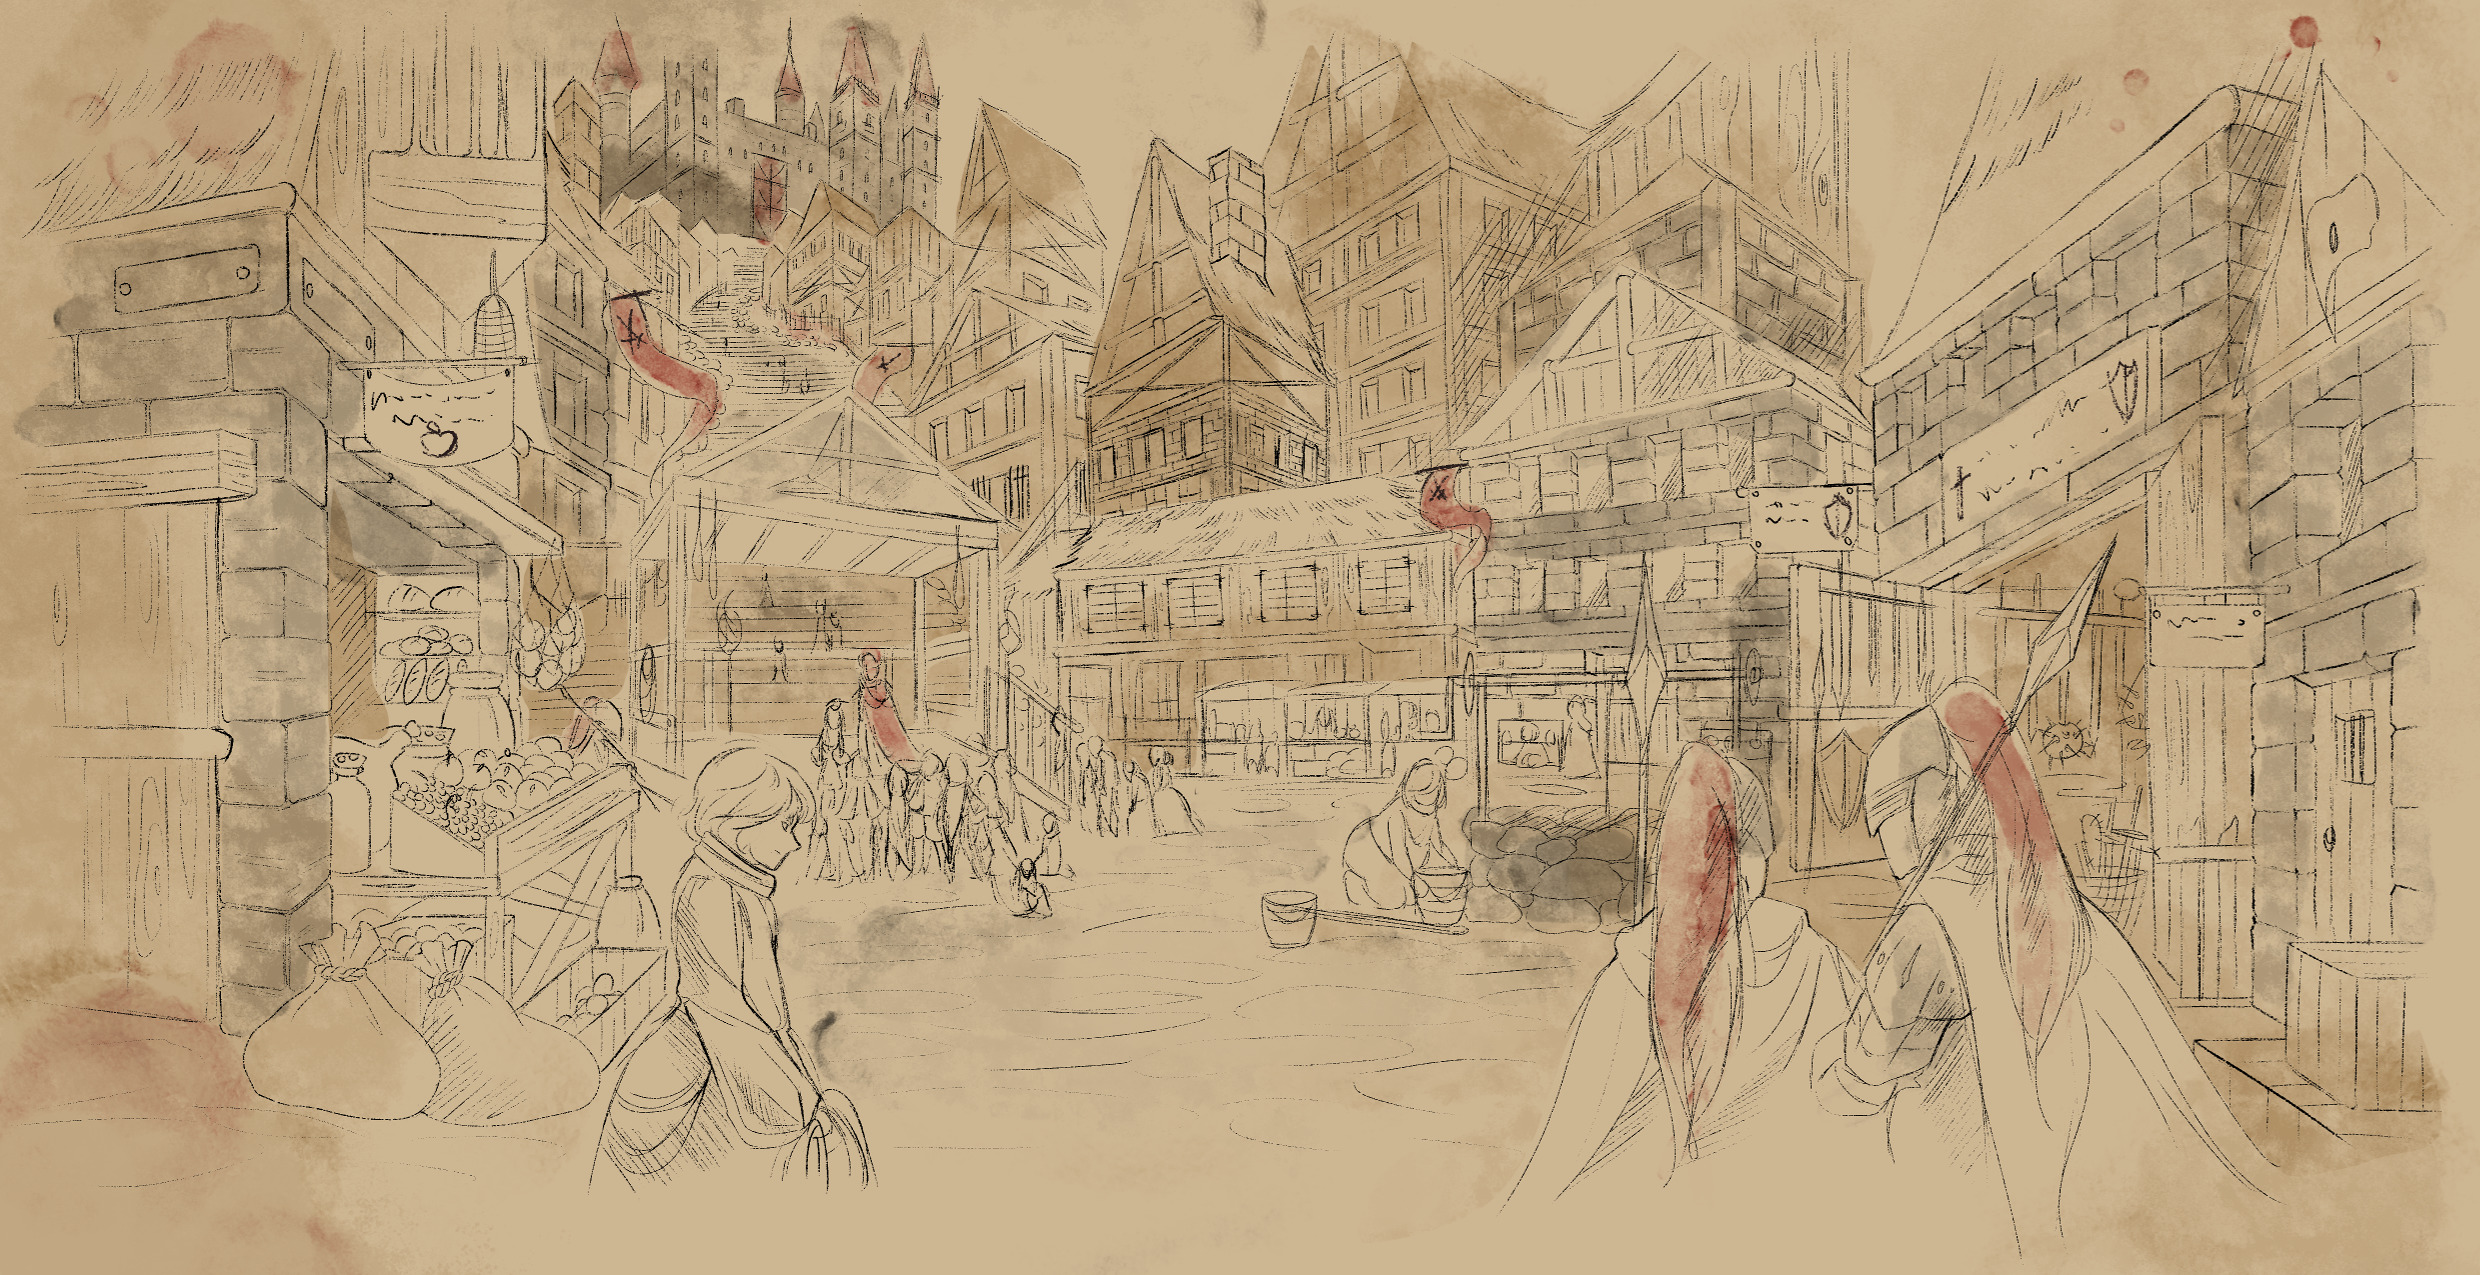
\includegraphics[width=\paperwidth,keepaspectratio]{media/norburysm.png}
  }
  \par
  Market place in \emph{Norbury}, circa GT:2102
\end{figure*}

\subsection{Norbury}
\label{sec:Norbury}

\graham{Surely the most vile city kingdom Aror has to offer...}
\aren{Bless thy innocent heart, for you have not lived long enough to see the
  rise of Morkan.}

The second youngest city kingdom, \emph{Norbury} resides on a large island off
the northern coast of the continent \nameref{sec:Eilean Mor}. Norbury is a
large walled city, encompassing a large part of the centre  of the huge island.

\subsubsection{History}

It was founded around \emph{GT:1849} as a joint military outpost of
\nameref{sec:Hraglund}, and other northern baronies of Eilean Mor. It was
originally intended as first line of defence against the many raids of the
beast races that came from the northern most continent of
\nameref{sec:Iafandir}. Quickly the fortress of Norbury grew into a castle,
and more and more people were required to keep the castle and its army
supplied. Armies need smiths, smiths need smelters, smelters need coal huts
and miners, and all of these need food, lodging and entertainment. Within a
few generations Norbury exploded in size and population, all working towards
one goal: keeping the raids and incursion of the beast races away from the
main continent.

By \emph{GT:2041} the city had surpassed baronies in sheer size and population,
and was granted the official status of a \emph{city kingdom}.

\subsubsection{Banner}

\begin{figure}[!ht]
  \centering
  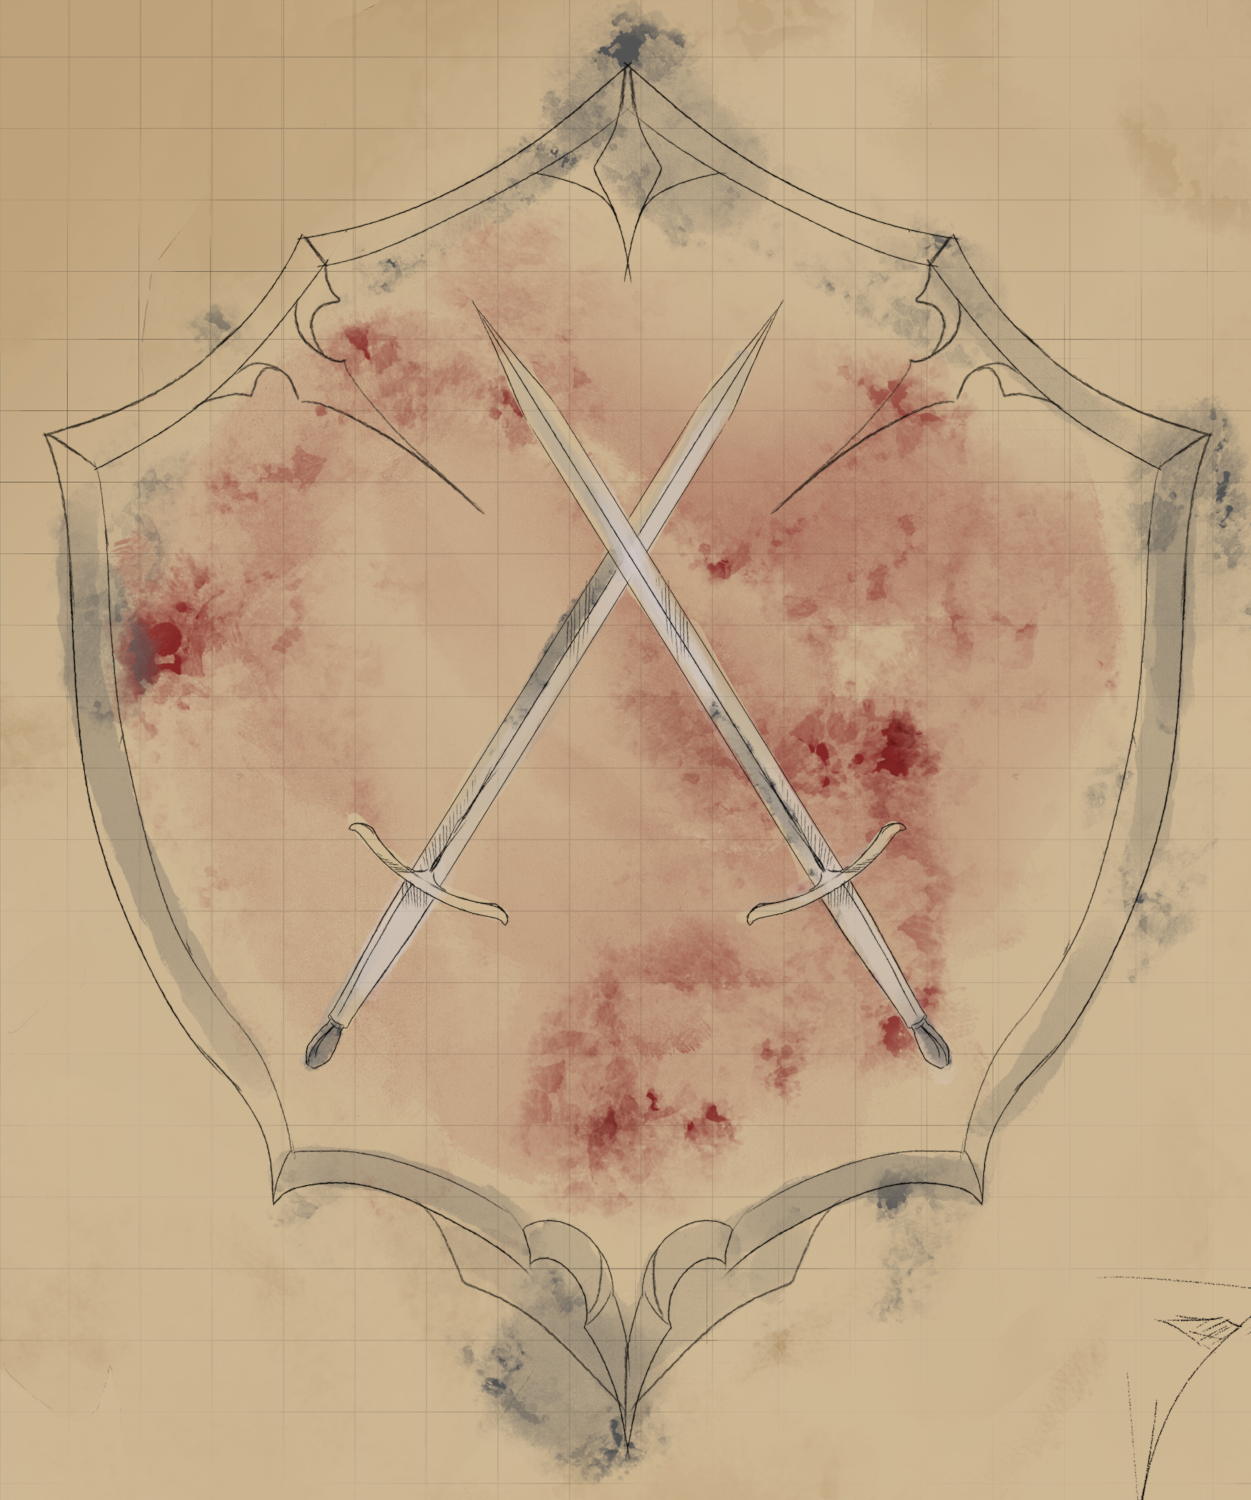
\includegraphics[width=0.9\linewidth]{media/norbury-bannersm.png}
\end{figure}

The kingdom's banner shows two silver swords crossed at the blade, against a
light red background. The main colours of the kingdom are silver and red.

\subsubsection{Districts}

The centre of the city is a large market place, with a big stone steeple in
the middle. The tower both signifies the eternal vigilance, but also houses a
large bell that is rung in case of an attack. Inscribed into the walls of
the steeple are the laws of the kingdom for everybody to read. The market
place is vast circular open courtyard, and all sorts of goods - including
slaves - are sold there.

To the north lies \emph{Norbury} castle, a huge fortified military camp and
seat of the monarch. It oversees the north eastern sea off the island, and
rests upon a roughly one hundred metre high cliff side. The castle district
also houses the richer barons, lords and ladies of the nobility of Norbury.

Further north west and south east lie the two major harbour districts that
the kingdom uses to maintains its vast fleet. Although these harbours are also
major trading hubs, they also house a majority of the city's working class or
poorer slaves.

To the south west lies the ``outreach'', a sprawling suburban district in which
the bulk of the Norbury citizens life. Both rich, poor, worker, artisan and
slave share this vast cityscape and life there together. Even though it is
called the ``outreach'' or ``outskirts'' this suburban area is still within
the city walls.

The surrounding area of the walled city houses farms and smaller villages that
also belong to the city kingdom. These farms are not walled, and thus
exposed to surprise sea raids from smaller vessels. The city provides these
outlying farms with watchtowers, patrols and sometimes even with full army
support are thus rarely defenceless.

In \emph{MI:1910} Norbury expanded its territory onto the mainland of Eilean
Mor. After the coastal barony surrounding castle Rothorn fell into disarray
when their old baroness died, the city kingdom invaded and claimed the land.
Norbury now holds and owns a small patch of costal area at the northern foot
of the \nameref{sec:Great Divide}.

\subsubsection{Sea Raids}

A network of watch towers, light houses, guard towers and scout ships
constantly check the sea north of \nameref{sec:Eilean Mor} for any impending
sea raiders that embark from the continent of \nameref{sec:Iafandir}. If a
suspicious ship or raiding party is discovered, the entire kingdom goes on
high alert and deploys their fleet. Norbury are excellent ship builders,
sailors and warriors on the sea; and so they prefer to capture and destroy
raiding parties before they land on Eilean Mor. Most of the ships manned by
the beast races of \nameref{sec:Iafandir} are often inferior in design, and
thus unfit for prolonged sea battles. Many are sunk off the coast of the
continent. The raiders that survive are fished out of the sea and then brought
back to Norbury.

There is a common misconception that Norbury enslaves all raiders that land
at the shores of Eilean Mor. But the city only enslaves those that actively
attack them, or raid coastal villages and towns as a way to make the raiders
repay the damage they have caused. Those that sail from \nameref{sec:Iafandir}
unarmed, or surrender, are more often than not escorted back to the savage
lands.

Sometimes raiding parties do sneak past the ever vigilant eye of the city,
and then land on the northern shores of Eilean Mor. Most of the baronies
on the shores have increased their armies to repel these raids upon their
lands. Yet some also call the mainstay army of Norbury for aid. Then the
soldiers of the barony attempt to bar the raiders from entering their land,
while the ships and navy of Norbury attack the landing party from the sea.

Defending Eilean Mor (the ``home land'') from sea raids is a cultural goal and
ideal, that is extended to any barony on the main continent. Some warriors of
Norbury even see it as impolite to ask for compensation or gold in exchange,
as there is enough honour already in defending their brethren of the main
land. Still many baronies and smaller earldoms pay Norbury for their aid,
either in gold, everblack or in trade deals highly favouring Norbury. Rivalries
that the city kingdom might have with the neighbouring baronies will not
hinder it to come to their aid in case of a raid from the sea.

\subsubsection{Religious Civil War}
\label{sec:Religious Civil War}

Ever since its foundation, the religions surrounding \nameref{sec:Lor}, the
\nameref{sec:Order} and the \nameref{sec:Three Kings} vied for the position of
dominance within the city. The Order had the most followers, followed by Three
Kings and then Lor. Although the priests and paladins of Order raised issues
with mistreatment of slaves, they were not outright against slavery unlike
the priests and followers of Lor who wished to see the practice banned. The
followers of the Three Kings found both the followers of Lor and the Order to
be weak in the face of their common enemy from the north, and were ready to
expel both religions from the city. Over centuries this conflict hardened and
brewed in the heads of the followers and citizens. Then, in \emph{MI:1480}
when a follower of the Three Kings beat his slave to death with a pavement
stone in the middle of the market place for disobeying him, a paladin of Lor
interfered by killing the slave owner in single combat. This event brought a
spark to the already volatile mix of religious animosity. The followers of the
Three Kings moved in retaliation against the temple and followers of Lor. The
Order, who sided with the mistreated slave, joined the conflict on the side of
the followers of Lor. A religious civil erupted that war lasted for two
months, in which both the Order and the followers of Lor suffered heavy losses,
and ultimately defeat, against a well-trained, well-equipped force inferior in
numbers. To prevent the bloodshed to spilling over to civilians, the then
ruling queen \emph{Arianna of Nordholm}, banned the religions associated with
Lor and the Order, and exiled their followers for being ``weak in the face of
adversity''.

Even though this conflict has long passed, the prevailing attitude in Norbury is
that followers of the Order and Lor were, and are still, weak and not worthy
of honour. Although the ban is still in place, the exile has since been
lifted, allowing priests and paladins of the two gods to visit the city.

\subsubsection{Culture}

Since the incursion and raids of the beast races still occur to this day, and
have grown to be more ferocious and demanding, the culture of Norbury has
grown in response. Norbury is from the lowliest slave and peasant up to the
king or queen herself, a meritocracy. You are worth as much to the city, and
in the eyes of your fellow citizen as you can contribute to the well being of
the entire whole.

Men and women of Norbury pride themselves in the work they are contributing to
the collective defence effort, be it front line combat, creating weapons and
armour for those that do, or aiding the effort in an administrative
fashion. Warrior culture runs strong in the kingdom, their deeds are sung in
taverns, and their likeness is made eternal in art. Many fighters and warriors
of Norbury follow the \emph{Three Kings}, although worship of \emph{Forun} is
also wide spread in the kingdom.

Although arcane and divine magic is still frowned upon in the kingdom, the army
of Norbury runs an academy for battle mages and wizards. Arcane research is
often scrutinized by its potential military application, and wizards are also
required to undergo basic military training in weapons and armour.

All citizens of Norbury (and those that wish to become citizens) must complete
a mandatory civil service of at least five years. Many use this mandatory
service to begin an apprenticeship, while others join the military to counter
raids and incursions. No one is excluded from this service, not even the
children of the reigning monarchs. Avoiding this service is not only illegal,
but is also seen as a major dishonour.

\subsubsection{Society}

Titles within the kingdom's society, such as commoner, earl, baron or even
duke and grand duke can be bought by any citizen of Norbury. There is a rather
unusual twist: These titles are not inherited, which means that the son of a
duke is a commoner upon birth. The common census is, that this child has not
done anything yet to earn the rank of earl for him or herself. There is a high
pressure on children to achieve the same status as their parents, or perhaps
even outperform them. Failure is always an option as well, as it is not
unheard of for a noble son to fall into slavery.

Who reigns as king or queen is decided in a ritual combat between all eligible
arch dukes that wish to rise to the challenge. This combat is not to the
death, although many grand duke's have perished in their claim for the
kingdom. A king or queen reins until his reign is challenged by another, or
until they die or resign. The people of Norbury mostly do not care what race
or social background of their king or queen, but instead judge all their peers
by their honour, combat prowess, and contribution to society as a whole.

\subsubsection{Slavery}
\label{sec:Slavery in Norbury}

Norbury is the foremost kingdom to practice slavery on a massive scale. Both
\hyperref[sec:Indentured Servitude]{indentured servitude} and
\hyperref[sec:Unregulated Slavery]{chattel slavery} are encoded in Norbury
law.

Many of the raiders that are captured, and most of those that commit major
crimes are enslaved. The wizard academy has constructed special
\hyperref[sec:Slave Band]{arcane collars} that bind the slave to their
owners. Slavery is rarely a sentence for life, as there are a few legal ways to
escape slavery. Slaves may be released at any time by their owners, those in
indentured servitude may buy themselves free, and state-owned slaves may be
simply set free once they can no longer contribute in any meaningful way to
society. However Norbury slaves (as compared those in servitude) have no
rights whatsoever, and are marked, colour coded, registered by number, and
tracked down by the \nameref{sec:Hunters Guild} should they decide to
run. Slave collars allow slave owners to track, command and often punish their
wearers.

Foreigners are allowed to purchase slaves, however they have to pay an
additional fee half the slave's value. This was intentionally done, so that
most of the slaves remain within the city and contribute to the city. Slave
ownership is recognised as lawful in all kingdoms and baronies that have
signed the \hyperref[sec:Vonir Accord]{Vonir Accord}.

Although the city has a large slave population (between 20 and 30 percent),
it rarely faces slave revolts or uprisings. There are four main pacifiers at
work that keep the slave population suppressed and obedient. First, for many
slavery is potentially only temporary. Many are forced to join the Norbury
army, the Hunter's Guild or begin work in other positions that would qualify
them for citizenship later on, and thus do not wish to risk their permanent
freedom through revolt. The second is a ever permeating culture of honour and
duty, especially in the still ongoing sea raids from the north. Many slaves
derive a sense of purpose from working toward a common goal. Also many
churches and charitable organisations provide a network of services and goods,
such as food, warmth and medical services to slaves making their lives
bearable. Although gatherings of slaves are forbidden, the Hunter's Guild
often looks the other way in regard to slave bars or inns, as long as no
direct threat stems from these establishment. And the fourth reason is the
ever vigilant \nameref{sec:Hunters Guild}. Their network of informants,
hunters, and agents quench any rebellious flame that might kindle in the dark.

\subsubsection{Spinetails}
\label{sec:Spinetails}

However the city also has a certain societal class of slaves that have slipped
through the crack of the Hunter's Guild. Those are slaves that were deemed
valueless, cannot work because of disease, illness or handicaps, are mentally
unstable or even violent, or may have lost their owner and thus no one lays a
claim on them. Their collars often show the colours ``white'' (valueless) and
``red'' (without owner), and are thus often named ``spinetails'' after the
bird that wears the same colours in its feathers. Spinetails hide within the
vast sprawling suburbia of the city from the guild, and survive by committing
petty crimes, begging or from aid given to them by generous people and
organisations. They have since begin to form their own societies, subculture
and even their own crime organisations. The Hunter's Guild warns anyone from
claiming a spinetail as a slave, and rewards citizens should they turn them in
or give hints that lead to their apprehension. Generally spinetails are viewed
as a problem by most citizens, and most owned slaves. Disease, drug abuse, and
crime is rampant within Spinetail subculture, and many see them as free-riders
and slackers.

\subsubsection{Population}

Norbury, and its outlying villages, houses roughly 4 million people. Of which
the vast majority are human and deepkin (39\%), then elves (24\%) followed by
dwarves (15\%) and half races (10\%). The rest (12\%) are beast races, almost
all of which are enslaved. Roughly 31\% of the entire population is either
currently enslaved or in servitude.

%% City Kingdom of Stenheim
\cleardoubleevenemptypage

%% TODO: Artwork

\begin{infobox}{City Kingdom of Stenheim}
  %% TODO: Crest
  \begin{multicols}{2}
    \begin{itemize}[label={},noitemsep,leftmargin=0.0cm,topsep=0pt]
      \infoboxitem{Location}{North western shores of \nameref{sec:Goltir}
      }
      \infoboxitem{Languages}{Doresh, Teranim, Old Teranim}
      \infoboxitem{Government}{Absolute Monarchy}
      \infoboxitem{Major Religions}{\nameref{sec:Forun}, atheism}
      \infoboxitem{Area}{est. 60,000 $km^2$}
      \infoboxitem{Population}{est. 19 million people}
      \infoboxitem{Non Grata}{monstrous races (including Gorgons), druids,
        devils
      }
      \infoboxitem{Magic}{All forms of magic overseen by the government, who
        grants permits and sets limitations
      }
      \infoboxitem{Slavery}{outlawed, indentured servitude available as an
        option to criminals to reduce sentence, imprisons criminals
      }
      \infoboxitem{Special Laws}{only state that allows sentient golems to
        become citizens
      }
      \infoboxitem{Notable Organisations}{\nameref{sec:House Ranian}, remnants
        of the ancient Deepkin houses
      }
      \infoboxitem{POI}{Central market, university of applied sciences and
        engineering, mountain plateau that is a recreational park, largest
        telescope on the northern hemisphere
      }
    \end{itemize}
  \end{multicols}
\end{infobox}

\clearpage

\subsection{Stenheim}
\label{sec:Stenheim}

The city kingdom of \emph{Stenheim} (also ``Stoahom'' in some local dialects)
lies on the north western shores of \hyperref[sec:Goltir]{North Goltir},
situated on the foot of the coastal mountain range of the Aldenes, where the
Taraun river flows into the sea. While the majority of the newer city has been
built at the foot of the mountain, the old city centre, the castle and main
fortifications reside in natural and hewn caverns in the mountain.

The city's banner features a red dragon upon a white shield, crowned by a
three pronged red crown. Red and white are the nations colours, representing
the iconic skin and hair colour of the \nameref{sec:Deepkin}.

\subsubsection{History}

It was officially recognised as a city kingdom in GT:1551, but is considered
far older. Earliest record dating back to almost GT:531 were found in the
vault of the city, albeit it was but a small deepkin settlement back then. It
began as a small tribal city, but soon the favourable conditions of the
settlement's location, namely access to the shore and fresh water from the
river, attracted more and more deepkin, and dark elven clans. Unlike most of
the dwarven clans that lived in the Aldenes, the deepkin clan welcomed their
surface brethren into their deep caverns from the beginning.

The deepkin built another smaller city outside their caverns, and used it to
trade the ores and gemstones to the other nations and kingdoms. The access to
the river, the easy connection to the sea (and thus trade), and its beautiful
and scenic lake scenery attracted more and more of the surface races, and the
city grew over the course of many centuries.

\subsubsection{Wars}

The kingdom was involved in many defensive wars over the course of its early
history. Many dwarven clans, especially the \emph{Black Hill} and
\emph{Snowhammer} clans, as well as remnants of the various Ilian empires of
the deep tried to seize the deepkin workshop. None of these assaults and sieges
was successful, and nowadays the kingdom of Stenheim has eclipsed all dwarven
and Ilian clans in size and power.

The deepkin had used their ingenuity to construct advanced war machinery such
as arcane siege weapons, arcane weapons and armour, as well as war golems to
defend their home. This distinct technological advantage helped them defeat
their aggressor, even though they often had superiority in numbers.  This
technological advantage did not sleep, and still to this day the city kingdom
is considered one of the strongest in terms of military power, capable of
fielding an army well equipped with arcane gear, as well as countless combat
ready golems, as well as arcane war and siege machinery.

Compared to many other more warring clans of the Aldenes, the deepkin never
enslaved or seized the lands of other clans. Most of the wars the deepkin
thought were defensive in nature. Their less aggressive approach, as well as
their propriety to get along, diplomatically and culturally, with the other
deep races made their kingdom an attractive destination for the other mountain
clans. Many smaller dark elven, and dwarven clans migrated to the city and
integrated well into the deepkin culture.

\subsubsection{Population}

The outlying city of Stenheim, as well as the deepkin workshop and castle holds
roughly 19 million people, of which the majority are deepkin (39\%) and dark
elves (22\%), while humans (11\%), elves (10\%), while halflings (4\%) and
dwarves (3\%) make up the minority. Due to the deepkin's liberal and welcoming
nature, Stenheim has become a destination for many half races (9\%) as well as
undead (2\%).

The city also uses humanoid-like golems for dangerous tasks such as city
defense, or difficult menial labour such as mining, construction or hauling.
They are called ``Homunkulus'' within the city, but outsiders know them mostly
from the many defensive wars where they earned the nickname ``Warforged''. The
vast majority of these golems are nothing more than well programmed, and
arcane automatons made of steel and Everblack. But some have gained
consciousness and self-awareness. Stenheim has retroactively freed and
liberated all self-aware Homunkulus from servitude, and given them citizen
rights within the kingdom.

Common male names are: Adrian, Alex, Andreas, Anselm, Arnold, Axel, Baldur,
Benjamin (Ben), Björn, Eckbert, Eduard, Erik, Erwin, Felix, Florentin
(Florian), Franz, Gisbert, Gregor, Gustaf, Heinrich, Helfried, Johannes
(Johann, Hannes), Karl, Klaus, Kilian, Lars, Leo, Lukas, Matthias,
Maximilian (Max), Nicklas (Nick), Oliver, Othmar, Patrick, Rafael, Reinhold,
Samuel, Sieghard, Sigismund, Torben, Valentin, Wolf

Common female names are: Abigail, Ada, Adelina (Lina, Adela), Alexandra (Alex,
Alexa), Amelie, Anna, Brigitte (Birgit), Daniela (Nela), Edit, Eleonora,
Elisabeth (Elisa, Elli, Lisa), Emma, Eva, Evelyn, Hanna, Helena, Ida, Ina,
Irene, Irma, Jana, Julia, Karla, Katarina (Katrin), Leah, Magdalena (Lena),
Margareta (Greta, Grete, Gretchen), Manuela, Mia, Ria, Rita, Roswita, Sara,
Sofia, Verena, Viola

\subsubsection{Culture}

The deepkin of Stenheim (and by extension the other races living there as
well), are predominantly atheistic. Only Forun and the other holy mothers have
a sizeable following within the mountain kingdom. The city mostly focuses on
mining and arcane research, and the people of Stenheim pride themselves for
being a centre for scientific and arcane learning.

Most people of the kingdom are considered humble, curious and known for their
love all things science and engineering. The deepkin have shared their passion
for golem construction, mechanical and civil engineering with the other races
that joined them. Almost all people in the kingdom enjoy luxuries that no
other kingdom can offer, such as indoor plumbing, arcane light fixtures and
cheap commodities due to early attempts at mass production.

The culture of Stenheim is known for being one of the most liberal and
advanced of all the city kingdoms. The people enjoy a wide variety of social,
economical freedoms, as well as a fair, stable and efficient state and legal
system.

\subsubsection{Rule}

The kingdom is lead by a patriarch or matriarch which is elected by council of
city elders, guild leaders, high ranking professors from the arcane academy,
as well as constabularies that are chosen by the general population through
votes. This ruler is then sworn in, and stays in power until his or her death,
abdication or until the council elects to vote for a new patriarch or
matriarch. Although not technically a queen or king, the ruler of the city is
deemed equal to a king or queen by the other city kingdoms and welcomed as
such.

More unusual is the fact that the kingdom is split into smaller districts,
each ruled by a constabulary. Although these local rulers report to the
matriarch or patriarch, they hold considerable power within their district,
and are even allowed to pen local laws. They are voted into office by the
people of their district, albeit the matriarch can remove a constabulary from
power.

The city's population and the majority of their rulers are against slavery,
and has also removed indentured servitude in favour of imprisonment. Convicted
criminals can still opt to reduce their sentence by mining for ore, or reduce
their sentence even further by mining for \nameref{sec:Everblack}. The kingdom
did not sign the \nameref{sec:Vonir Accord}, but most of their citizen are
well protected from slavery in other kingdoms as no foreign power wishes to
risk a diplomatic incident with Stenheim.

\subsubsection{Relations}

The kingdom holds good relations with the other city kingdoms, except for
Kesmar. Stenheim often accused the dwarven kingdom for secretly aiding their
enemies during past sieges and skirmishes. Most of surrounding dwarven clans
in the mountain hold the kingdom in contempt, seeing them as an imperialistic
force with no equal in power. Even though the kingdom does not aggressively
expand, the surrounding clans and tribes are pressured into joining the city
or face becoming irrelevant next to their neighbour.

Furthermore Stenheim is known for exporting both their advanced war machinery,
technology, ore and everblack to other nations. It is known for selling their
weapons and golems to anyone who are able to front the price.

%% City Kingdom of Tredegår
\subsection{Tredegår}
\label{sec:Tredegar}

The city kingdom of \emph{Tredegår} (old-high Teranim for ``three courtyards'')
lies on the south western shores of \emph{Eilean Mor} west of the \emph{great
  divide}. It is encased by two large rivers: The \emph{Morre} river to the
north and west, and the \emph{Moy} river to the east and south. It's close
proximity to the mineral wealth of the great divide, the easy access to two
rivers and the sea made Tredegår one of the richest city kingdoms of all of
\emph{Aror}.

\subsubsection{An'Rath}

In the centre of the city is the vast castle of \emph{An'Rath}, which houses
roughly a thousand people. Workers, nobles, clergymen, bureaucrats, judges,
advisers, as well as the ruling family live within the castle. The castle by
itself is an impressive architectural feat, and is constantly being extended
with additional towers and buildings. The castle has its own army, and its own
inner stone wall for protection, and even inner draw bridges and gates to
separate individual parts from one another in case of a siege. The outer ring
of the castle is open to the public, and houses a library, a school that
offers various courses, its own brewery and tavern (\emph{The Drunken Trader}).

\subsubsection{Banner}

The banner of Tredegår features a white tree with three thick branches resting
within a shield. A golden crown rests above the shield. Gold, white and blue -
representing the gold of the great divide, the white snow up on their peaks,
and the blue rivers and the sea - are the colours of Tredegår.

\subsubsection{Population}

Among all the city kingdoms Tredegår is by far the biggest. It houses roughly
32 million inhabitants, with all the outlying villages included. Most of these
are humans (55\%), with dwarves that once lived in the great divide following
close second (21\%) followed by elves (10\%), half races (12\%) and various
others (2\%).

\subsubsection{Culture}

The immense wealth of the city has trickled down to most of the lower and middle
class citizens. Thus the people of Tredegår live in an unparalleled state of
social security that is only known in that kingdom. Most people of the city
work far less than their contemporaries in other kingdoms. Still they make
enough money to life comfortably. This gives the people of Tredegår time and
opportunity to enhance their education and other skills. The people of Tredegår
are often described as well educated, easy going and relaxed; with strong focus
on self improvement and family. Some have described them as arrogant and snobby,
although those attitudes can often be exaggerated by envy. A typical Tredegår
craftsman for example works slow, meticulously and prefers to deliver quality
over quantity. This culture of ``do it right; or do not do it at all'' has
earned the city a good reputation as a reliable trading partner that delivers
excellent product.

This culture is also present within the kingdom were houses, streets, bridges
are seldom derelict or run down. Instead they are always lavishly decorated with
flowers, and the city maintains a network of arcane street illumination housed
in lamp posts. Public workers keep the streets clean and make sure that the
city always Although the city as no slum or worker district, poverty does
still exist within the city, especially among the sick and crippled.

\subsubsection{Steel and Smithing}

The \emph{Tredegår Steel and Gold Corporation} is one a large company that
runs many forges and smithies across the city. It works off the raw ore mined
either in the great divide, or ore that has been brought in from the
\nameref{sec:Silver Isles}. The corporation is known for its excellent
craftsmanship in weapons and armours, and their products are sold all across
the major kingdoms and are renowned for their quality and steep price.

\subsubsection{Society}

Without the economical pressure due to the immense wealth of the city, slavery
has been abolished several centuries ago. The city has been ruled by the same
noble family \emph{Gylleborg} for thousands of years. Both female and male
heirs may rule. The city kingdom has a long history of peace and prosperity,
and the justice system is known all around the world as one the best of its
kind. Independent judges and prosecutors work in tandem with private defence
attorneys to ensure the justice system remains fair and independent.

\subsubsection{Relations}

The city and its nobility is closely related to \nameref{sec:House Ranian},
and the house has the main headquarters near the main square of the city.

Due to their status as rich trading partner, the city kingdom of Tredegår is
in good standing with almost all other city kingdoms, except \emph{Morkan}.
Their longest standing trading partner and ally is the city kingdom of
\emph{Fes al-Bashir} to the south. The city kingdom strengthened their bond
with the other city states by providing logistical advisers, money and
their best smiths during the rebuilding of \emph{Forsby}. The kingdom is a
signer of the \emph{Vonir Accord}.



% Regions of Aror
\section{Regions}
\label{sec:Regions}

Although civilisation can mostly be found in the large city kingdoms, it does
not mean that the more rural areas are filled with savages. Many big regions
share similar cultures or backgrounds, and it is not uncommon to find people
that have moved out of their city kingdoms into these areas. Either to start a
simpler live as farmers, or because a business opportunity or the love of
their life has drawn them there.  Likewise many people move from the country
side to the big cities in the hopes of finding better opportunities, such as
jobs and education there.

The following chapter of this book should introduce you to several regions of
Aror. Their culture, their believes, as well as their struggles and victories.
Tread carefully in these regions, as you might find friend and foe alike.

%% Dirgewood
\subsection{Dirgewood}
\label{sec:Dirgewood}

The \emph{Dirgewood} is a vast forest south east of the \nameref{sec:Great
  Divide}, a large mountain chain that splits the continent of
\nameref{sec:Eilean Mor} in half north by south. It runs along most of the
southern side of the Great Divide, reaching up the mountains until the tree
border, but does not extend to the shores. It is a vast temperate and boreal
forest and marshland, that is split by a few major rivers that have their
origins in the Great Divide. The thick woods, harsh and unwelcoming marches,
and hilly terrain has made it almost impossible to build large castles in the
Dirgewood. However it is dotted with thousands of smaller towns and villages.

The Dirgewood is mostly settled by humans, wood elves, snow elves, and
halflings. The hilly regions of the Dirgewood are also home to deepkin, and
dark elves. Many monstrous tribes remain, especially hobgoblins, bugbears,
kobolds and goblins as well as many tribes and packs of lycanthropes. The
Dirgewood is also known for still housing many faeries and fey. The Dirgewood
is one of the few areas in which the \nameref{sec:Aeon of Strife} is still
actively fought between humanoid and beast races.

Albeit the humanoid villages are as diverse as any city they have two things
in common: Most villages know of each other, and even know people from other
villages. They trade with each other often, intermarry, and also come to each
other's aid in case of an attack. Most of the time they fight monstrous races
and beasts, but have also killed bandits that settled in their land or halted
the expansionist dreams of baronies that board the Dirgewood. Skirmishes,
feuds and even wars between the villages are known to happen, but are far and
few in between.

The other thin in common is a staunch belief and adherence to the tradition of
the \nameref{sec:Old Ways}. Almost all villages are lead by a village elder, a
shaman, and a war chief. Most villages and small hamlets celebrate the rituals,
incantations, spells and sacrifice demanded by them by the three (or four)
mothers, and view outsiders that do not believe in the old ways as
suspect. They harbour an open animosity against anyone that would follow a
lesser deity. This animosity is rarely violent, except to those that would
come to the Dirgewood as missionaries.

Although the old traditions are part of their religion and culture, there
exist a great variety in how they are followed among the various tribes. Some
are more strict than others, and while others only revere three mothers, other
revere four and in turn those are split on who the fourth mother truly is. But
most tribes have forgone with the oldest, most brutal traditions. For example
very few tribes still practice humanoid sacrifices to \emph{Marwaid}, or do so
extremely rarely. The Old Ways, and their interpretation within the Dirgewood
and Golian Heights is the birth place for modern equality among men and
women. During the aeons of conflict with the beast races everyone is
encouraged to follow his or her inner calling (or ``true will of the mothers''
as it is often referred to), and thus contribute to the family, village or
town to the best of their ability.

The many rivers that flow from the mountains to the south-eastern shore lines of
\emph{Eilean Mor} are used to transport people and goods in and out of the
Dirgewood. The villagers use the river network to trade with each other, raid
monstrous encampments and tribes, as well as communicating and trading with
the large city kingdoms that reside on the shores of Eilean Mor.

For many city dwellers that follow the three goddess' of the old ways, the
Dirgewood is a popular destination for a pilgrimage and spiritual
enlightenment. The people of the Dirgewood are known to be highly spiritual,
and to them the stories, spirit worship, chants and spells of Old Ways are
part of their daily lives. They welcome any humanoid species that also follows
the Old Ways, or at least one of the three mothers, and adheres to their rules
and customs.

The people of the Dirgewood are known as hardy survivors, expert hunters,
fierce raiders, and proud warriors, and above all else spiritually enlightened
people that take great care in preserving their aeon old traditions and
believes. They dress in plain clothes, but take great pride in elaborate
jewellery made out of bone, antlers, animal teeth, precious metals or
gemstones. To combat, a hunt, or ritual ceremonies they also wear detailed
white, grey or blue face and body paint. The body paint acts as camouflage,
but also to intimidate their enemies.

Common male names are: Aeron, Aled, Andras, Arwyn, Bryn, Cadell, Dylan,
Eirian, Gareth, Glyn, Eifan, Ivor, Maldwyn, Owain, Rhys, Tegid, Wyn

Common female names are: Aerona, Anwen, Bethan, Blodwen, Branwen, Cadi,
Catrin, Deryn, Eira, Elin, Gwendoline, Gwenith, Llinos, Mairwen, Nia,
Siana, Tegwen, Wynne


%% Farou Island
\subsection{Farou Island}
\label{sec:Farou Island}

\emph{Farou Island} is a huge island off the east coast of
\nameref{sec:Arania}, and used to be the original home of the dragons, before
they moved east onto \nameref{sec:Draigynus}.

Farou contains a central mountain range, which is also called Farou. The
mountain range gives birth to many rivers, which in turn feed thousands of
smaller lakes, which again feed the islands vast and impressive tropical flora
and fauna. The island is simply known as the ``savage jewel'' by most humanoid
cultures, as its stunning beauty is only darkened by the feral beasts that
roam its jungles, and swamps.

The ancient dragons that first settled Aror made this island their home,
building housings, research labs, vaults, temples and even draconic cities on
its surface. After the giants followed them onto Aror, the island was the main
battle ground between these two ancient extra-planar species. Even though the
dragons won, many buildings, temples, and laboratories were destroyed during
the conflict, and now exist as ruins on the island. A specific mountain in the
Farou range is simply called the ``dragon grave'', as many dead dragons have
been buried on its steep slopes, and in its crevasses. After the core humanoid
races emerged on Aror, the dragons moved further east as to avoid interfering
with their natural development.

Slowly nature regained control of the island. Very few humanoid settlements
exist there, and most are expeditions of \nameref{sec:Fes al-Bashir}, that
have established harbours on the island's coast. Although the island is
mostly free of dangerous monstrous creatures, the thick vegetation, harsh
swamps, and treacherous and often unstable dragon ruins, make exploration
a dangerous endeavour.


%% Kanaria Archipelago
\subsection{Kanaria Archipelago}
\label{sec:Kanaria Archipelago}

North of \nameref{sec:Karnak} lies a vast archipelago called the Kanaria
Archipelago. A vast collection of small and large islands that stretch out
into all directions. These islands share the same humid climate as most of
Karnak and are thus tropical paradises, with white beaches, palm trees, clear
water and covered with thick and lush rainforests. This paradise is only a
façade however, as most are inhabited by various tropical beast races, such as
hydras, or nagas, or tribal humanoids, and medusa, that are fiercely
protective of their islands.

As one of the few remaining frontiers, many explorers travel to the archipelago
in the hopes of discovering new land, islands, riches and gold. The waters
however are often treacherous, the island inhabitants dangerous and many
unsavoury groups. Slavers and pirates operate out of bases hidden in the
silver isles, preying on the native population, and passing ships alike.

Nevertheless the islands are known for harbouring many exotic plants, fruits,
and herbs, such as tobacco, chocolate and coffee. While the mountains and
volcanoes of the isles are filled with silver, gold, and
\hyperref[sec:Everblack]{everblack}. The trading companies of many large city
kingdoms have outposts and colonies on the isles, and often bitterly rival
over these resources. This brings them in direct conflict with the humanoid
tribes of the isles, called the \emph{Inua} who they often exploit, displace
or even enslave.

\subsubsection{Inua}
\label{sec:Inua}

The Inua are several native humanoid (halfling, dwarven, elves as well as
human) tribes that have lived on the islands of the archipelago since the last
ice age. Inua generally have darker skin, a stout and strong build due to their
reliance on heavy labour, and their own language called \emph{Inue}. They live
in tribes or small towns, and are excellent hunters, gatherers, and boat
builders. They often travel around the archipelago to hunt, fish, or to raid
other Inua tribes that dot the islands.

They often wear minimal clothing made out of fur and hide, and use crude and
primitive weaponry made out of stone, bone and wood. Very few Inua tribes have
mastered weapons out of metal, such as iron or even steel. Their appearance is
often frightening, as they enjoy piercing and tattooing themselves, especially
with white or other bright colours. Nevertheless they have a long, and rich
tradition and history, most of which is shared orally. The Inua are known to
be excellent warriors, cunning huntsmen, deeply spiritual, and communal people.

They are staunch believers of an entity they call \nameref{sec:Isamir}.
He tells them to honour the sea, the lakes, and all things that dwell within
them. He is said to conjure storms to cleanse islands, but also to grant
smooth weather so that the Inua can fish. He demands sacrifices of his people,
and they often sacrifice large catches they make, and sometimes even go so
far to sacrifice members of other tribes or foreigners to him. In recent years
however the worship of \nameref{sec:Isamir} has been challenged among the
Inua. Worship of \hyperref[sec:Forun]{Elora} (the ``lady of fire'' in Inua)
has become widespread, as she grants divine power, warmth and does not require
living sacrifices to be made to her.

Still the Inua are known for building secret temples in the jungles of their
islands. These temples are holy places, where no foreigner is allowed to
tread, and thus they are often guarded by mummified undead that the shamans of
the Inua create and command. These undead were once strong and proud warriors
that now fulfil the last great honour of the Inua: defend the holy sites
against intruders for all eternity. The Inua are expert embalmers, and their
shamans are renowned necromancers, and often also worship \nameref{sec:Morana}.

Although proud and strong warriors, the Inua are not as developed in terms of
technology as the rest of the humanoid that come to the archipelago. Even
though they more technologically primitive than the humanoid races of the city
kingdoms, their fierceness in battle, expert skill in stealthily attacking
with small manoeuvrable boats, unparalleled knowledge of the islands, and
their necromancer shamans allowed them to resist many invasions and
attacks. Some tribes have suffered defeat by the hands of the expeditions that
came to the islands, and have thus become wary, secretive or outright
xenophobic. Some tribes openly trade with the foreigners to their islands, in
hopes of making alliances or friends, while others are openly hostile and will
scare off or kill anyone that dares to set foot on their islands.

The Inua are in a constant battle against the foreigners that come to their
islands in the hopes of exploiting their resources. They openly wage sea
war against slavers, pirates and ships of trading corporations that seek
to displace them to gain access to their wealth.


%% Pale
\subsection{Pale}
\label{sec:Pale}

Toward the far north, past the \nameref{sec:Cnamh Mountains} lies the northern
pole, and down south, far beyond the deserts and steppes of \nameref{sec:Arania}
lies the southern pole. Both are vast desolate lands covered in snow and ice,
and are commonly just referred to as the \emph{great pale}.

Both poles are harsh climates, reaching temperatures below 50 degrees Celsius
during the night. Inhospitable to most life forms, only a few specially adapted
creatures such as ice bears, penguins, sabre tooth tigers and woolly mammoths.

\subsubsection{Tribal Snow Elves}
\label{sec:Tribal Snow Elves}

The pale is also the home to the tribal \hyperref[sec:Snow Elves]{snow elves},
often called \emph{elves of the pale}, or \emph{pale elves}. These names are
also used to differentiate the tribal snow elves from those that live in
cities and nations.

They live in small families, or together in small clans and best the bitter
cold better than any other sentient race. Their physique makes them naturally
resistant to the extreme cold, and they have produced some of the finest
archers and hunters that can hunt, track and kill even the most dangerous game
found in the pale. Pale elves have developed special methods to construct
their \hyperref[sec:Snow Elf Bow]{special hunting bows}, that are now sought
after all across the world.

Pale elves prefer to remain on the move, and roam the pale wastes as nomads.
They value their own community and family above all else, but are a strictly
patriarchal society, where only men may lead the tribe. Women may not assume
any dangerous activities within society, such as being a huntress or warrior,
and thus often become priestesses, gatherers or remain with the children. It
is also customary to gift younger females off to other tribes, often without
their saying or choice in the matter, in an attempt to bring the roaming
nomadic tribes closer together.

While the more civilised nations and states, as well as the snow elves living
within them, would laud and look down upon these tribal structures and
traditions, they are just that: Old and tried traditions that have ensured the
survival of the snow elves for centuries. Some tribes have broken with these
traditions, allowing women to pursue a more active role in society but these
are far and few between. Such change if often necessitated by a shortage of
able bodied men, good hunters, or a lack of a male heir to the tribal
chieftain, rather than actual pursuit for equality within the tribe.

Tribal pale elf tradition is communicated through stories of great ancestors,
and their noble and selfless deeds. And it is exactly those ancestors that the
snow elves revere and pray too. However those stories also contain
supernatural beings, especially an aspect of \nameref{sec:Forun} as the all
mother of life and patron mother of snow elves, as well as a trickster aspect
of \nameref{sec:Isamir} that serves as her foil. Isamir is not evil in these
stories, however he assumes the role of a trickster deity.

To tribal snow elves the community, family and their own tribe is everything, as
it ensures survival and in the frozen tundras. The harshest punishment within
these communities, reserved for major crimes, is exile which is often equal to
a death penalty. Since these exiles are then also shunned by other snow elven
tribes, they sometimes wander away from their homes and join city kingdoms or
baronies.

Furthermore many slavers attempt to move into the frozen waters of the pale
in the hopes of capturing and enslaving tribal snow elves. These expeditions
are extremely dangerous and many slavers have perished to the cold, dangerous
beasts or the expert archery of the snow elves.


%% The Great Divide
\subsection{Great Divide}
\label{sec:Great Divide}

The continent of \nameref{sec:Eilean Mor} is split in half, from the north west,
to the south east, by a large mountain chain called the \emph{Great Divide}.

Many dwarven, deepkin and especially dark elven clans call the mountains their
home, and have built small underground cities and settlement in the vast caves
of the mountain chains. The mountains are also known for being home to many
beast races, such as tribes of orcs and goblinoids.

Many rivers spring forth from the massive glaciers that top the great divide,
feeding hundreds of lakes as well as making the land fertile both to the north
and the south. South of the great divide lies a vast boreal forest called the
\nameref{sec:Dirgewood}.

The mountain chain has not only divided the land in half, but has also been
a major divider on the continent in the culture of the people. Since the north
of Eilean Mor has no major city kingdoms except \nameref{sec:Tredegar}, it has
always been viewed as more uncivilised than the southern region. This of
course holds no longer true, but that sentiment is still stuck with the people
of the south. So much so that the phrase \emph{``north of the divide''} has
become a moniker to denote someone who lacks manners.

Still the mountain range is a huge geographical obstacle, and only a few
dangerous mountain paths lead safely through the mountains. Since these paths
are often waylaid by monstrous bandits, rarely anyone ever crosses these
mountains, unless they absolutely have to. Most of the baronies and small
cities north of the great divide instead trade with the south, and the rest
of the world, through the sea.

The northern tip of the great divide is currently claimed by
\nameref{sec:Norbury}, who owns and operates a large castle in the mountain
range called castle \emph{Rothorn}. The castle oversees several mining
operations based in the mountain range producing ore such as copper and silver
for the kingdom.

The southern end is owned by \nameref{sec:Tredegar}, and is heavily mined
by various dwarven clans for the city kingdom. The iron and adamantine ore
from the mountains is heavily used by the kingdom to make excellent arms and
armour.


%% Silver Isles
\subsection{Silver Isles}
\label{sec:Silver Isles}

In the centre of the vast sea that separates all continents lies a vast
archipelago called the \emph{Silver Isles}. A large collection of small
islands that stretch out into all directions, and are loosely connected to the
continent of \nameref{sec:Goltir} by a land bridge. Almost all of the islands
either lie on, or very close to the equator of \hyperref[sec:Aror]{Aror}. Most
are thus tropical paradises, with white beaches, palm trees, clear water and
covered with thick and lush rain forests.

While not technically a city kingdom, the region itself holds vast power,
both politically and commercially. The islands are rich with all manner of
natural resources, including silver, iron, copper, gold and Everblack. The
people of the isles (often simply called ``islanders'') have organised
themselves by establishing many large cities with vast trading empires,
as well as smaller ports, harbours and settlements all around the archipelago.

\subsubsection{Masia}
\label{sec:Masia}

These settlements are numerous, but one large harbour port sits in the centre
of it all: Masia. With about 400,000 citizens it is the largest, most
prosperous of all the harbour towns of the isle. It is not recognised as
independent as it is partially owned by the \nameref{sec:Ror-Aram Trading
  Corporation}, with \nameref{sec:House Ranian} holding a large stake in the
settlement. The city is thus ruled by a steward, that oversees that the city
turns a profit for the trading corporation. The city is known as haven for
smugglers, pirates, slave trade, but also for unfathomable riches, in which
all sorts of luxury goods - such as tobacco, cigars, coffee and chocolate, are
sold.

Common male names are: Agustin, Alfonso, Alsen, Alvaro, Benito, Damian, Diego,
Enrique, Felipe, Gabriel, Garcia, Leon, Manuel, Martin, Ramon, Salvador, Tello,
Valeriano, Ydalla

Common female names are: Ana, Angel, Clara, Elena, Elvira, Fatima, Felipa,
Francisca, Gracia, Juana, Luzia, Manuela, Olalla, Serena, Ynes, Ysabel

\subsubsection{Fleeting Alliances}

Most smaller harbours, and port towns are usually independent ventures that
live off their agricultural products, as well as mining the mountains of
the islands for their riches. Their allegiances, political, cultural and
commercial significance vary greatly over time, and many attempt to sabotage
their competitors or even try to expand their operations by taking over other
islands. Some do it through the vague veil of threats, sabotage and political
intrigue, while others do it through threats, violence and outright war.

The major players involved in the region are Ror-Aram Trading Guild, House
Ranian, the \nameref{sec:Velvet Hand} as well as the mysterious
\nameref{sec:Silver Hand}. Thus some ports are nothing more than slaver
holdouts, while others are smuggler ports or straight out pirate havens.

Even though the area is often in disarray due to political chaos, struggle our
outright conflict between varying factions, the people of the isles have often
proven that they can work together should the need arise. As was the case during
the Devil siege of \nameref{sec:Forsby}, when the islands offered their highly
secured bays and harbour facilities as a staging ground for a counter strike.
Many of the native cities and ports, including Masia, even joined the counter
attack and provided valuable resources, weapons, experienced sailors and ships.

Keeping the smaller ports and harbour towns separated and in constant
conflict, unable to rally around Masia to form a kingdom, is the main goal of
the larger city kingdoms, \nameref{sec:House Ranian}, and the various trading
guilds involved in the area. The divide and conquer tactics have been
successful in keeping the people of the isles from becoming a major power on
Aror for several centuries.


%% Suam Desert
\subsection{Suam Desert}
\label{sec:Suam Desert}

The \emph{Suam Desert} (suam is Gnoll for ``sea of fire'') is a vast sand
desert in the heart of the continent of \nameref{sec:Arania}. With scorching
temperatures averaging between 30, and 40 degrees it is a place hostile to
most forms of life.

The desert is dotted with small oases, which allow limited vegetation, and
fauna to survive the scorching temperatures of Aror's biggest hot desert.
Few humanoids traverse, or live in the desert. The desert is mostly inhabited
by gnolls, who see the Suam Desert as their holy birth right. Although the
oasis would allow for other humanoids to settle, very few do so, as the gnolls
drive everyone off their holy land. Apparently a large surviving settlement
of \nameref{sec:Ilians} live beneath the Suam Desert in a vast network of
sandstone tunnels. These Ilians have fled there from all around the world,
and live beneath the gnolls in secrecy.

The desert does contain a few natural sandstone mountains, valleys and
cliffs. These often contain oases at their basin, as the natural barriers
catch, and collect rain water. Many of these valleys are thus popular with
the local flora and fauna, and their cooling shade provide respite from
the scorching heat of the overhanging suns.

Both the desert, and its inhabitants are actively avoided by humanoids of
Arania, preferring to use ships and teleporters to circumvent crossing the
desert in its entirety. This sentiment is mostly shared by the gnolls of
the desert, as they rarely wander towards the coast, which are primarly
inhabited by the core humanoid races.


%% Toralian Highlands
\subsection{Toralian Highlands}
\label{sec:Toralian Highlands}

The \emph{Toralian Highlands} (``Toral'' or the ``Highlands'') are a vast
stretch of land in the centre of \hyperref[sec:Goltir]{North Goltir}. It
stretches from the borders of \nameref{sec:Forsby} in the west, all the way east
towards the \nameref{sec:Cnamh Mountains}. North east of Toral lies the
mountain range of Alpara, and to the south west the region borders the Walusian
desert. Most of the region is boreal or temperate, with many places covered
in ancient forests, harsh swamps and marches, but also vast stretches of
fertile grass land and plains. The Highlands also contain two of the biggest
lakes in Aror: at the centre lies \emph{Ledava}, and to the north west lies
lake \emph{Ferto}.

Much like the \nameref{sec:Dirgewood}, the difficult terrain, and the ever
constant threat of the beast races (such as orcs, goblins and hobgoblins)
makes settling Toral a dangerous endeavours. Very few humanoid baronies exist
within the region, and most of the Highlands is settled by smaller tribes,
villages, or perhaps the odd city. Life in the Highlands is harsh and
unforgiving, as the monstrous and humanoid races still fight over land,
resources, and culture to this very day. Many wild and fantastical creatures
call the region their home, and fey and druids still roam the secluded places
of the Highlands.

Much like the Dirgewood, many of the Highlanders are staunch followers of
the \nameref{sec:Old Ways}, and form small settlements lead by warlords,
shamans, and village elders. Within Toral, the people still believe that
\nameref{sec:Morana} is the fourth mother, and her worship as a goddess of
winter, death and rebirth never waned. Many shamans of Toral practice
necromancy, and vampires are a common sight within the tribes and villages.
They welcome any humanoid, half-humanoid or vampire that follows the Old Ways,
or at least one of the mothers. The lesser deities have little power or
following within the region.

Culture and tradition is particularly kept well in line between the Dirgewood
and the Highlands, although scholars did not know how for quite a while. Until
it was discovered that the ancient \hyperref[sec:Tynrikke]{Týn} connected most
of their ruins through teleportation magic, allowing seamless travel between
the Dirgewood and the Highlands. This was a secret kept by shamans of both
sides, and was used to facilitate that, but also to allow for an escape route
in case villages or tribes were threatened.

\aren{It's not ``until it was discovered'', it is ``until I, Graham Balance,
  discovered''...}
\graham{Now, now. Let's avoid bragging, and keep the book professional.}

The politics of the Highlands is ever shifting, with many villages, towns
and cities either aligned or at odds with each other. The constant battles
and skirmishes between the monstrous and humanoid races contribute to an
ever shifting landscape, into which even the most powerful kingdoms of the
regions, namely \nameref{sec:Forsby}, \nameref{sec:Kesmar} and
\nameref{sec:Stenheim}, rarely interfere.

Common male names are: Aleks, Anton, Bogdan, Boris, Dejan, Dusan, Emil,
Gal, Janosh (Janos, Jan), Jaromir (Jaro, Mir), Milan, Miklos, Nikola
(Nikolaus, Nikolai), Radek, Soma, Stanislav (Standa), Viktor, Zdisa

Common female names are: Anna, Abigel, Bianka, Brana, Elisabeth (Elsa, Lisa),
Elena, Emma, Emelie (Amalie), Helene, Johanna, Lucia, Magda, Malina (Melina,
Lina), Melinda (Linda), Mira, Nada (Nadia, Nadezhda), Radmila (Mila), Rosalie
(Rosa), Sobena, Svetlana (Lana), Vera, Vesna, Zvesdana (Zvesda)


%% Yua'cata
\subsection{Yua'cata}
\label{sec:Yuacata}

Yua'cata is a vast rain forest on the main land of \nameref{sec:Karnak}. It is a
wild and savage place, untouched by civilisation. The rain forest surrounds the
vast fresh water lake of \emph{Mu'ut}.

Yua'cata is home to thousands of different species of animals, such as birds,
insects, reptilians as well as predatory felines and snakes. The warm climate
and the abundance of water and resources lead to a diverse and large biome.

\subsubsection{Mu'ut}
\label{sec:Muut}

\emph{Mu'ut} is a large fresh water lake in the centre of the continent of
Karnak. It is geologically active, and its warm water fuels thousands of
smaller and bigger rivers that flow in all directions towards the sea. Mu'ut
can be considered the heart of the Yua'cata rain forest, as its warm waters
fuel the tropical climate, rain and thus the vast rain forest of Yua'cata.

\subsubsection{Tribes}

The jungle is also inhabited by thousands of tribes of sentient monstrous and
humanoid races, including humans, \hyperref[sec:Wood Elves]{wood elves},
\hyperref[sec:Medusa]{medusa}, as well as lizardfolk and sahuagin. Most of
these are hunters and gathers, and often differ greatly in traditions, customs
and believes. There is one cultural element that many tribes share however: an
almost holy reverence of the lake of Mu'ut.

\subsubsection{Savage Elves}
\label{sec:Savage Elves}

The most notorious of the jungle tribes are the wood elven tribes of the
Xanarian river. Among other races these wood elves are often referred to as
\emph{savage elves}. They worship an ancient being called \nameref{sec:Xir}
who they believe sleeps beneath the surface of the holy rivers of Mu'ut. Xir
teaches that all unbelievers are impure, and can only be redeemed by feeding
them to him by drowning them in the river. These wood elves raid, pillage,
murder and sacrifice other sentient races they come across without mercy, as
in their eyes there is only one way for them to be redeemed in the eyes of
their lord.

The Xanarian tribes also practice cannibalism. They believe that eating their
own kind after death makes their deceased continue to live within them. They
rarely eat outsiders, as they believe their flesh to be corrupt and impure.



% Local games
\subsection{Games}
\label{sec:Games}

If you ever wander into a local establishment you might be interested in
joining the locals for a game of cards. This section of the book will explain
the rules of the most commonly played card games on Aror, but be aware that
local variants and house rules are common as well. Also be aware of cheaters,
and those that seek to exploit your inexperience to pluck your money right
out of your pocket.

\subsubsection{Kratzen}
\label{sec:Kratzen}

Kratzen (Reatham for ``scratch'') is a card game popular in
\nameref{sec:Forsby}, as well as the \nameref{sec:Toralian Highlands}. It is
played with 4 to 6 players.

The game is played with a deck of 32 cards, that come in four distinct
colours: hearts (red heart), diamonds (bells), spades (green leaf), and clubs
(acorns). The cards ranking is: Mother / Sow > King > Queen / Ober > Jack /
Unter > Ten > Nine > Eight > Seven. However the seven of diamonds (bells),
also called the \emph{Weli}, is considered the second highest card, just beneath
the mother of the trump.

At the very beginning each player pays the minimum bet. The dealer must pay
the minimum bet again before dealing any cards. The dealer then deals out two
cards to each player, before giving himself an open third card that determines
the colour of the trump. If the open third card is the \emph{Weli}, then the
dealer must make a choice: Either they bless it with another card (whose
colour becomes the trump colour), and they automatically take on the role of
the \emph{striker}, or they forgo blessing in which case the \emph{Weli} turns
into a regular seven of diamonds, losing its status of the second highest
card. After the trump colour has been determined, the dealer gives two
additional cards to other players, and themselves.

Now the next player in line must make a statement regarding their role in the
game: \emph{Pass} means that the player does not wish to make a
statement. \emph{Or} means that the player will beat the game with a different
colour as trump, and \emph{strike} declares that the player is capable of
winning the game. A player who wishes to bid must outbid the players before
them, for example a player can declare ``or'', but could be outbid by the next
player who declares a \emph{strike}. If every player passes then the cards are
shuffled again, and the next player deals. Don't forget to pay the minimum bet
as a dealer.

If no one overrules an \emph{or}, then the dealer must openly deal cards until
a new trump colour has been chosen. This new card is given to the one who
declared the \emph{or}, and they become the \emph{striker}. Now that a
\emph{striker} has been chosen (either by an \emph{or} or because one player
declared a strike), all others have a chance to either \emph{come along} (play
against the striker), or \emph{stay at home} (skip the game). All those that
\emph{come along} must make one trick, and the \emph{striker} must take two
tricks. If no one plays against the \emph{striker}, then the \emph{striker}
automatically wins the pot.

Then any players still in the game, starting with the \emph{striker}, must
reduce their hand to four cards, and may exchange up to three cards from the
talon. The \emph{striker} is allowed to dismiss three cards, and buy four new
ones from the talon by openly presenting the Mother of the trump colour should
they have it in hand. Once all players have reduced their cards to four, the
\emph{striker} plays the first card, and the other players must play the same
colour if they have it (Farbzwang). If they don't have that colour they must
beat it with a higher trump card. They may add any card if they don't have the
colour, or can't beat the highest card in play. The player that makes the
trick is next in turn to play the first card, and game continues until four
rounds in total have been played.

Any player who \emph{came along} must score one trick to win, and the
\emph{striker} must secure two tricks to win. After all tricks have been made
the pot is divided into four parts, and each player with a trick receives a
part of the pot. The remainder goes to the \emph{striker}. If a player has
\emph{fallen} (i.e. failed to gain at least one trick), they must pay current
amount of the pot into the next pot. If the striker has \emph{fallen} (i.e.
failed to secure at least two tricks), then they must pay double of the
current pot into the next pot.

\aren{And now you know why people call this game ``one step above robbery''
  as the pot has a tendency to grow exponentially.}

Many variant rules exist, for example in some games a dealer can opt to simply
reshuffle, and hand over dealership to the next person should their trump card
be a seven of hearts, spades or clubs. Other games allow players to purchase
an ``arse'', in which they discard three cards, present the forth openly, and
receive three new hidden cards. A fifth card is then dealt to them openly, and
should that card be a trump, more open cards are dealt to them until they
receive a non-trump card. Many friendly, and low-stakes games simply limit the
amount of money losers have to pay into the pot. Other games have a
\emph{pass-or}, which is ranked lower than a regular \emph{or}, in which only
one card is revealed and its colour becomes the new trump colour. This of
course has the risk of leaving the trump colour unchanged.


% Characters
\section{Characters}
\label{section:Characters}

% Aren Fel
\subsection{Aren Fel}
\label{sec:Aren Fel}

Aren Fel of \nameref{sec:Nicte}, most commonly known as the ``Undying Witch''
(born sometime around GT:24) is a \hyperref[sec:Deepkin]{Deepkin}
\hyperref[sec:Soul Magic]{soul witch}, priestess of the \nameref{sec:Silent
  Queen}, thief, diplomat, author, historian and scholar.

Her family tree, blood line, birth and association with House Nicte have been
thoroughly documented and dated to GT:24. She was born to small deepkin
commune, which now lies within the kingdom of \nameref{sec:Stenheim}. And even
though she possess new female deepkin bodies to stay alive over the aeons, her
continued longevity as been independently confirmed by several other
long-lived species, including vampires, dragons and even giants, who were able
to recognise her unique soul across the centuries.  This is also why her
appearance is not described, as it would be a fruitless labour.

Initially born into the Nicte family clan, she was trained preliminary as a
diplomat, thief, spy and trader. As the battles of the aeon of strife came
closer to her family, she was also hastily trained in combat, and joined the
skirmishes as an archer and scout. She suffered a major trauma and wound during
those skirmishes, which also \hyperref[sec:Soul Awakening]{broke her soul}.
After her clan realised her condition, Aren was sent off to be healed by the
\nameref{sec:Walburga} witches. Aren took the opportunity to learn as much as
she could about soul magick from them, including how to possess other people
or bodies. Although she was inducted into the coven as a witch, she was
ultimately asked to leave due to her allegiance to a lesser deity. Aren still
uses this power by possessing newer, younger bodies to prolong her life.
Although the races she inhabits now vary, she always remains female.

During her unnaturally long life-span she used her extensive
training from her Deepkin clan to forge alliances, gather artefacts,
manoeuvre political developments, and to manipulate the rich and powerful.
She consolidated many smaller baronies, bolstered their political and military
power, and directly steered many of them to join or start wars that would see
an end to the strife on Goltir. Aren achieved this goal over the course of
several centuries by holding high ranking offices, such as adviser to the baron
or baroness. She was thus instrumental in the early history of the
north-western part of \nameref{sec:Goltir}, by making sure the core humanoid
settlements remained allied with each other. Aren was instrumental in paving
the way for both Stenheim and \nameref{sec:Forsby} to rise to be global
powers.

She was also heavily involved in the \nameref{sec:Holy Crusade}. There she
managed to lessen the extend and cruelty of the crusade by actively opposing
the persecution of low-ranking followers of Griannar, including the general
congregation and low-ranking acolytes. Aren directly stood against her own
high-priestess \nameref{sec:Aria}, causing a schism within the church of the
\nameref{sec:Silent Queen}. Between the warring faction following Aria on one
side, and the more neutral, and pacifist congregation that followed Aren, on
the other. Aren further aided \nameref{sec:Hraglund} during the plague, and
assisted the kingdom in finding a cure by securing the help of important
arcane institutions including the \nameref{sec:Hall of Knowledge} and
\nameref{sec:Magistrata Arcanum}. The last recorded appearance of Aren was
during the siege of Forsby, where she smuggled \nameref{sec:Everblack Golem}
made by Stenheim into the city to help with the defence against the devils.

Although her achievements are well recorded, so are the means by which she
attained them. Aren is notorious for her Machiavellian scheming, and often
pursuing careless and reckless plans, in which she prioritises a quick and
satisfactory end of the crisis at hand above anything. Her philosophy that the
ends justify the means, has lead to her to commit blackmail, theft, slavery,
and even murder. She is often accused of showing a blatant disregard for the
lives of others, for example by killing the souls of future hosts simply to
extend her own lifespan, or by deliberately starting wars during the
strife. Her many, and well documented crimes, has made her an enemy of many
judicial organisations, such as the church of \nameref{sec:Lor}, or the church
\nameref{sec:Order}. She is furthermore a persona non grata in four city
kingdoms: Fes al-Bashir, Forsby, Hraglund, and Tredegår.

\label{sec:Witch Hunt}
The power she wields, both literally as a powerful soul witch, and
figuratively through her web of alliances, caused a lot of animosity and open
hostility from other powerful organisations. In MI:20, after the Holy Crusade,
the \nameref{sec:Knight Order of Tavos} attempted to catch, trial and execute
Aren. A literal witch hunt began, that lasted from MI:20 to MI:28 that caused
many innocent Deepkin women harm, caused them to lose their freedom and even
their lives in an attempt to bring Aren to justice. This is period of time is
now known as the ``Witch Hunt'', and is considered the sole fault of the Knight
Order of Tavos.

Nevertheless her knowledge of the world, its inhabitants, the creatures and
threats of the planes, arcane, and soul magic is extensive, as is her web work
of power, alliances, and ability to influence even the most powerful
organisations. As a member of \hyperref[sec:Two Courts]{Court of the Suns},
she is very often asked for aid, when a global crisis afflicts Aror.

\begin{note}
  Aren can serve many purposes in your campaign: she can be the secondary
  villain, prime villain, or simply be an aid to the party, preparing them
  to face the actual villain. She will \emph{never} work towards the doom of
  Aror, or its citizens on purpose, but will use \emph{whatever means
    necessary} to achieve goals. Even though these goals may overlap with
  that of a good PC party (i.e. saving the world), her methodology and
  philosophy make her an evil character in terms of D\&D alignment.
\end{note}

\begin{35e}{Aren Fel 1 Fighter / 17 Rogue}
  \srditem{Size/Type}{Medium Humanoid (Deepkin)}
  \srditem{Hit Dice}{2d10 + 15d6 (79+36) 115 HP}
  \srditem{Initiative}{+3}
  \srditem{Speed}{30 ft.}
  \srditem{Armour Class}{}
  \srditem{BAB / Grapple}{+12/+19}
  \srditem{Attack}{}
  \srditem{Full Attack}{}
  \srditem{Space/Reach}{5 ft./5 ft.}
  \srditem{Special Qualities}{Dark Vision (120 ft.)}
  \srditem{Class Features}{Sneak Attack (+9d6), Trap Finding, Penetrating
    Strike (ACF), Improved Uncanny Dodge, Improved Evasion, Skill Mastery (Use
    Magic Device)
  }
  \srditem{Soul Power Points}{1d6+15d8 (80+144) 228 SPP}
  \srditem{Soul Powers Known}{All of them}
  \srditem{Saves}{Fort: +8, Ref: +10, Will: +5}
  \srditem{Abilities}{STR: 30, DEX: 16, CON: 14, INT: 16, WIS: 12, CHA: 26}
  \srditem{Skills}{Bluff (+30), Diplomacy (+29), Disguise (+19), Hide (+4),
    Intimidate (+21), Knowledge (local) (+21), Knowledge (Planes), Knowledge
    (Soul Magic) (+17), Move Silently (+4), Search (+19), Sense Motive (+19),
    Soulcraft (+17), Spot (+19), Tumble (+4), Use Magic Devise (+21)
  }
  \srditem{Feats}{1: Able Learner, 2: Improved Initiative, 3: Radiant Soul,
    6: Power Attack, 9: Craven, 12: Staggering Strike, 15: Combat Reflexes, 18:
    Robilar's Gambit
  }
  \srditem{Items}{Aren's Grand Seal of Nicte [Ring] (+10 Diplomacy, +10
    Bluff), Aren's Remembrance [Ring] (+8 Charisma, +8 Strength)
  }
  \srditem{Challenge Rating}{18}
  \srditem{Alignment}{Lawful Evil}
  \srditem{Advancement}{Rogue levels}
\end{35e}

% Eigyr
\subsection{Eigyr}
\label{sec:Eigyr}

Eigyr Waylin (born circa GT:-550, and died circa GT:-320) was a high elven
warlord, politician, shamaness of the \nameref{sec:Old Ways} that rose to
prominence in her campaign against the monstrous races on \nameref{sec:Eilean
  Mor}.

Her history, deeds, accomplishments but also most of her defeats and failings
are well documented in the stories, songs and traditions of the Old Ways. Within
humanoid traditions and culture of both the Eilean Mor, and the northern part of
\nameref{sec:Goltir} she is universally celebrated as a heroine, champion and
liberator. Her fame also stretches across the continents, and her tactics and
teachings have also been extensively studied by the scholars of Arania and
Avenfjord. Eigyr's fame turns into notoriety among the monstrous races, who see
her as conqueror and defiler of their lands.

In her early years she was an accomplished huntress, archer, and wielder of
two blades in each hand, and fought the monstrous races by leading small war
bands, and employing mostly hit-and-run tactics. Through many early victories,
and skilled diplomacy she rallied more and more villages and tribes behind
her. Soon she had a formidable army, and began to assault, and besiege larger
monstrous towns. Eigyr lost many of these earlier large scale battles, as she
failed to adapt tactics, and logistics from the small skirmishes she knew well,
to tactics and logistics required of a large and vast armies. Her pride and
bullheadedness are often attributed to those seemingly needless losses.  After
appointing new advisers, and generals to lead her ever growing armies the winds
turned again in her favour. She is remembered as a woman who fought with
honour and courage in battle, never taking lives of the innocent (be they
beast or men) and actively punishing her men and women if they committed war
crimes against the innocent.

Eigyr is described by many stories as a wise, natural, honour-bound and
charismatic leader, but also as a spiritual purist. She detested the worship
of lesser deities, especially the \nameref{sec:Three Kings} but also those of
\nameref{sec:Lor}, and \nameref{sec:Griannar}. The stories tell, that she often
refused to aid those that worshipped ``false gods'' or those that she felt were
without honour.

Her campaigns ended around GT:-390, after she had defeated all major monstrous
cities on Eilean Mor, and driven most monstrous tribes across the northern sea
to \nameref{sec:Iafandir}. Eigyr ruled wisely and justly over her newly formed
empire in the centre of Eilean Mor until her death. In her final years she
also often travelled her empire, telling her own story to the people. Eigyr,
becoming wiser in her years, never failed to mentioned her failings and lost
battles, urging people to learn from them. She especially regretted the
needless losses in the early sieges, brought on by her inability see that she
could not lead and oversee the grand army all by herself.

Many towns, villages, cities and even \hyperref[sec:Wayfaerers
  Guild]{organisations} are named in her honour, although her empire fell
apart soon after she departed. Most large humanoid city kingdoms and some
baronies of Eilean Mor owe their founding to her legacy. Also many of the
newer traditions of the \nameref{sec:Old Ways} are directly based on her
teachings, and retelling of her own story in her later years.

% Graham Balance
\subsection{Graham Balance}
\label{sec:Graham Balance}

Graham Balance, born GT:2084 somewhere in the Dirgewood, died GT:2139 in
\nameref{sec:Fes al-Bashir}, was one of the great polymaths of early Arorian
history. He was an accomplished writer, musician, historian, philosopher,
arcane wielder, politician and grand magus of the hall of knowledge.

As a young adult Graham travelled around the world, from his home in the
Dirgewood across the sea to Goltir, all the way down south, across Farlar, and
then met the dragons of Draigynus, before finally settling Arania. On his
pilgrimage across the world of Aror he penned the most popular, and most
widely printed and copied book on all of Aror: the ``Wayfaerer's Guide to
Everblack''. He also penned most of his other popular works, specifically songs
and poetry, both the originals, and those he collected from various cultures
around the world, on his year long journey. His songs are still sung today,
and his rhymes and words are still recited to the next generation so they are
not forgotten.

After arriving in \nameref{sec:Fes al-Bashir} he joined the \nameref{sec:Hall
  of Knowledge}, were his broad knowledge of the world earned him a teaching
position. As a professor for cultural history, ancient societies and languages
he taught several student generations, before deepening his understanding of
arcane magic, philosophy and science. It was at the academy where he wrote his
greatest work: ``The History of Divine Form'', which is a detailed treaty and
look on the old religions, true deities and their teachings. It also put forth
a hypothesis: that if enough people believe in a true deity, one might be
``willed'' into existence. It is in this book were he founded a new religion
and dogma, with another true deity at its centre: the \nameref{sec:Sea
  Priestess}.

After about fifteen years of professorship he rose to be the Grand Magus of
the Hall of Knowledge, and thus, in turn, became the most powerful political
figure in Fes al-Bashir. He ruled the city and the Hall of Knowledge until his
death in GT:2139. Although his reign was short, he moved both the Hall of
Knowledge away from worship of lesser deities, and towards the sciences. And
although internal power struggles within the cities prevented him from
enacting lasting change in the city, he is still remembered as a wise,
tempered, and just ruler of the city.

Graham balance is mostly remembered when he was Grand Magus. As a man in his
advanced years, short hair, a beard that reaches down to his chest and covers
most of his face. He had sharp blue eyes, a long elongated face, and was
decently handsome. His charisma stemmed from his sharp and eloquent wit, as
well as his commandeering presence.

% Irene de'Var
\subsection{Irene de'Var}
\label{sec:Irene deVar}

Irene de'Var, Countess of Saremen, is the current ruler of \nameref{sec:House
  deVar} of Saremen in \nameref{sec:Helmarnock}, and thus one of the five
rulers that make up the council of the city kingdom.

Irene is about two metres tall, and has short white dyed hair, deep and dark
red eyes, and blue finger nails that show her usage of \nameref{sec:Ramesk}.
Her origin as a \hyperref[sec:Snow Elves]{snow elf} has granted her with
natural grace and beauty, which she complements with elaborate and intricate
silken garments, expensive and impressive jewellery (both magic and mundane)
as well as graceful posture and mannerism.

The countess is seen as a cunning politician, and a passionate and genius
orator capable of inspiring and moving their subjects through speeches, and
using her commanding presence and eloquence to resolve conflicts through
negotiations. To her people she shows her warmer, more compassionate side,
often meeting her own subjects on festivities or other special occasions.

Originally a snow elf diplomat of Helmarnock stationed in \nameref{sec:Forsby},
she was turned into a vampire in MI:1081 by the Count Nareil of House de'Var,
to serve as an heir in his lineage of nobility. His nobility has roots back to
the time of the great betrayal by \nameref{sec:Morana} during the aeon of
strife, and was instrumental in establishing and defending the city on the
island of Saremen amidst the constant wars and battles fought against the
beast races. Even though the countess has been trained in classical sword
fighting, and especially fencing, she prefers diplomacy over war and conflict.

Irene has ruled House de'Var since MI:1121 after the death of Nareil. She has
since restructured and reformed the House, leading them to become the most
dominant noble family on the island. Irene largely follows the houses traditions
and Nareil's teachings, and stays true to Nareil's style of leadership of
benevolence and diplomacy: Irene outlawed slavery on Saremen in MI:1122
freeing all who were previously enslaved to a citizen of Saremen, and pushed
the council to allow \nameref{sec:Umgeher} and \nameref{sec:Gorgons} back into
the kingdom. The ban on slavery was partially effective, since the city
kingdom has signed the \nameref{sec:Vonir Accord} before her push toward slave
liberation. Even though no new slaves may be taken within Saremen, and all
slaves of Saremen citizens have been freed, slavers of other nations,
including the other islands of Helmarnock are still allowed to follow that
practice on Saremen.  She initiated a council vote on slavery, but was
defeated two to three.

Generally Irene de'Var attempts to drive the society of Saremen towards
individualism, liberty and freedom, lifting many restrictions both in the
social sphere - such as lifting marriage restrictions between mortals and
vampires, ending slavery or allowing Gorgons to become citizens - as well as
in the economical sphere by lowering taxes and making it easier for companies
to do business. Her political leanings and open policies, together with her
well-received, compassionate speeches towards her subjects, have made her a
well beloved and respected countess among the citizens of Saremen. Although
she is a brilliant politician and orator, she keeps a cadre of highly skilled
advisers as a ``council of ministers'' that oversee other aspects of the
island, such as defence, finances, civil engineering or oversee the Academy of
Arcane Arts.

\begin{35e}{Irene de'Var (13 Bard / 2 Fighter)}
  \srditem{Size/Type}{Medium Undead (Vampire)}
  \srditem{Hit Dice}{15d12 (98 HP)}
  \srditem{Initiative}{+13}
  \srditem{Speed}{30 ft.}
  \srditem{Armour Class}{40 (9 dex, 10 armour, 5 deflection, 6 natural), 24
    touch, 31 flat-footed}
  \srditem{BAB / Grapple}{+11 / +17}
  \srditem{Attack}{+24 +4 Rapier 1d6+6 18-20x2}
  \srditem{Full Attack}{+24/+19/+14 +4 Rapier 1d6+13 18-20x2}
  \srditem{Space/Reach}{5 ft./5 ft.}
  \srditem{Special Attacks}{Blood Drain (Ex), Create Spawn (Su), Energy Drain
    (Su)}
  \srditem{Special Qualities}{Scent (Ex), Feral Blindness (Ex),
    Damage Reduction (Su), Resistances (Ex) DR 10 cold and electricity,
    Spider Climb (Ex), Turn Resistance (Ex) +4, Fast Healing (Ex)
  }
  \srditem{Class Features}{Bardic music, Bardic knowledge, Countersong,
    Fascinate, Inspire courage +2, Suggestion, Inspire greatness, Song of
    Freedom
  }
  \srditem{Spells Known}{\emph{Level 0}: Detect Magic, Fleeting Fame, Ghost
    Sounds, Dancing Lights, Prestidigitation, Read Magic

    \emph{Level 1}: Improvisation, Invisibility (Swift), Silent Image, Identify

    \emph{Level 2}: Alter Self, Detect Thoughts, Invisibility, Suggestion

    \emph{Level 3}: Blink, Haste, Dispell Magic, Halt

    \emph{Level 4}: Dimension Door, Freedom of Movement, Invisibility
    (Greater), Blinding Beauty

    \emph{Level 5}: Dispell Magic (Greater), Cacophonic Burst (Greater)
  }
  \srditem{Saves}{Fort +12, Ref +22, Will +26}
  \srditem{Abilities}{Str 22, Dex 28, Con -, Int 18, Wis 22, Cha 36}
  \srditem{Skills}{Bluff (+39), Intimidate (+41), Perform (Oratory) (+31),
    Perform (Dance) (+31), Diplomacy (+41), Gather Information (+31),
    Knowledge (Arcane) (+22), Knowledge (Royalty \& Nobility) (+22), Knowledge
    Local (+22), Sense Motive (+42), Spellcraft (+22), Hide (+17), Move
    Silently (+17), Search (+12), Listen (+14), Spot (+14)
  }
  \srditem{Feats}{Force of Personality, Leadership, Extend Spell, Metamagic
    Song, Improved Weapon Finesse, Improved Initiative, Weapon Finesse,
    Heighten Spell}
  \srditem{Items}{Royal Regalia of Saremen (+8 Charisma, +10 Armour Class),
    Seal of Saremen (+5 Resistance, +10 Diplomacy, +10 Sense Motive), Crown of
    Saremen (+5 Deflection AC, +10 Intimidate)
  }
  \srditem{Challenge Rating}{18}
  \srditem{Alignment}{Neutral Good}
  \srditem{Advancement}{By character class}
\end{35e}


